\documentclass[10pt, letterpaper]{article}
\usepackage{../../../template/template}
\usepackage{xspace}
\usepackage{float}
\usepackage[italian]{babel}

% ------------------------
% Impostazioni documento
% ------------------------

\setDocTitle{Manuale Utente}
\setDocVersion{0.2.3}
\setDocData{13/04/2026}
\setDocIndex{Manuale Utente}
\setDocState{1}
\setDocRecipient{2}

\newcommand{\user}{Utente\xspace}
\newcommand{\os}{Operatore Sanitario\xspace}
\newcommand{\admin}{Amministratore\xspace}
\newcommand{\cloud}{Cloud Vimar\xspace}
\newcommand{\reparto}{Reparto\xspace}
\newcommand{\appartamento}{Appartamento\xspace}
\newcommand{\myvimar}{MyVimar\xspace}

\newcommand{\screenshot}[1]{%
    \begin{center}
    \fbox{%
      \parbox{0.8\textwidth}{%
            \centering\vspace{1em}
            \textit{[Inserire screenshot: #1]}
            \vspace{1em}
        }%
    }
    \end{center}
}

\begin{document}

\makeTitlePage

\newpage 
\addChangelog{0.2.3}{13/04/2026}{F. Venzo}{G. De Fina}{\noOne}{Modifica sezione specifiche hardware e installazione}
\addChangelog{0.2.2}{10/04/2026}{V. Baleanu}{G. De Fina}{\noOne}{Aggiunta sezione riferimento API}
\addChangelog{0.2.1}{09/04/2026}{V. Baleanu}{G. De Fina}{\noOne}{Aggiunta sezione test}
\addChangelog{0.2.0}{06/04/2026}{L. Granziero}{G. De Fina}{\noOne}{Schermate di gestione, configurazione allarmi}
\addChangelog{0.1.0}{05/04/2026}{L. Granziero}{G. De Fina}{\noOne}{\firstDraft}
\makeChangelog

\newpage

\tableofcontents

\newpage

\listoffigures

\newpage

% \listoftables

% \newpage

\section{Introduzione}

\subsection{Scopo del documento}
Lo scopo del Manuale Utente è quello di introdurre il lettore al Sistema sviluppato da \textit{SnakeByte} per il Capitolato${_G}$ C9 proposto da \textit{Vimar S.p.A.}.
Il manuale illustra le modalità di installazione del Sistema e le operazioni che l'utente può svolgere all'interno del Sistema, guidandolo passo dopo passo nelle funzionalità disponibili.
\\In particolare, nel presente documento sono contenute le seguenti sezioni:
\begin{itemize}
    \item \textbf{Concetti}: una spiegazione completa dei concetti chiave che potrebbe essere necessario conoscere per utilizzare il Sistema correttamente;
    \item \textbf{Test}: una spiegazione su come eseguire i vari test di unità, integrazione e accettazione;
    \item \textbf{Requisiti}: una definizione di quelli che sono i requisiti minimi di \textit{hardware}, \textit{software} e \textit{browser} per poter correttamente eseguire il Sistema;
    \item \textbf{Accesso e installazione}: una spiegazione dettagliata per poter eseguire il Sistema;
    \item \textbf{Guida all'utilizzo}: una guida completa che descrive in modo chiaro e dettagliato le operazioni da eseguire per utilizzare una specifica funzionalità;
    \item \textbf{Supporto tecnico}: una sezione dedicata alla richiesta di assistenza in caso di problematiche durante l'utilizzo della piattaforma.
\end{itemize}

\subsection{Glossario}
All'interno del documento possono essere presenti termini il cui significato può risultare ambiguo o sconosciuto, essi sono
riportati in italico e alla loro prima occorrenza è associata una \textit{G} a pedice ad indicare la presenza del suddetto termine 
all'interno del \texorpdfstring{\textit{glossario}}{glossario}$_G$, che è disponibile al seguente link: \href{https://snakebyteteam.github.io/glossary.html}{Glossario}.

\subsection{Riferimenti}
\subsubsection{Riferimenti normativi}
\begin{itemize}
    \item \textbf{Norme di Progetto}:
          \\ \url{https://snakebyteteam.github.io/3-PB/Documenti_interni/Norme_di_progetto/Norme_di_Progetto_v1.0.0.pdf}
          \\ (consultato il 10/04/2026).
    \item \textbf{Vimar View4Life Capitolato di Ingegneria del Software Università di Padova 2025-2026}:
          \\ \url{https://www.math.unipd.it/~tullio/IS-1/2025/Progetto/C9.pdf}
          \\ (consultato il 10/04/2026).
\end{itemize}

\subsubsection{Riferimenti informativi}
\begin{itemize}
    \item \textbf{Analisi dei Requisiti}:
      \\ \url{https://snakebyteteam.github.io/3-PB/Documenti_esterni/Analisi_dei_requisiti/Analisi_dei_Requisiti_v2.0.0.pdf} 
      \\ (consultato il 10/04/2026).
    \item \textbf{Glossario}:
      \\ \url{https://snakebyteteam.github.io/2-RTB/Documenti_interni/Glossario/Glossario_v2.0.0.pdf} 
      \\ (consultato il 10/04/2026).
\end{itemize}


\section{Concetti}

\subsection{Tipi di utenti}
Nel Sistema realizzato sono presenti due tipologie di utenti: \textbf{\admin} e \textbf{\os}.

\subsubsection{Operatore Sanitario}
L'\textbf{\os} è l'utente che opera all'interno del Sistema svolgendo attività legate ai reparti e agli allarmi. Può consultare e aggiornare le informazioni di propria competenza, senza però avere accesso alle funzionalità amministrative.
Questo tipo di utente può effettuare le seguenti azioni:
\begin{itemize}
    \item Autenticazione;
    \item Prima autenticazione con cambio password;
    \item Visualizzare il cruscotto iniziale (\textit{Dashboard}${_G}$);
    \item Visualizzare e modificare lo stato dei dispositivi \textit{IoT}${_G}$;
    \item Visualizzare e risolvere gli allarmi attivi;
    \item Visualizzare lo storico degli allarmi risolti;
    \item Visualizzare l'elenco delle notifiche;
    \item Visualizzare il cruscotto analitico (\textit{Analytics}).
\end{itemize}

\subsubsection{Amministratore}
L'\textbf{\admin} è l'utente responsabile della gestione complessiva del Sistema, inclusi i reparti, gli allarmi e gli operatori sanitari presenti.
In aggiunta alle funzionalità disponibili all'\os, questo tipo di utente può effettuare anche le seguenti azioni:
\begin{itemize}
    \item Collegare il proprio profilo all'\textit{account} \textit{MyVimar};
    \item Visualizzare, creare e gestire le regole di allarme;
    \item Creare un reparto;
    \item Assegnare degli appartamenti ad un reparto;
    \item Assegnare degli Operatori Sanitari ad un reparto;
    \item Creare ed eliminare utenti di tipo \os.
\end{itemize}

\subsection{Reparti}
Raggruppamenti logici di appartamenti e operatori sanitari, 
che rispecchiano l'organizzazione della struttura. 
Ogni reparto ha un nome, un insieme di appartamenti assegnati e un 
insieme di Operatori Sanitari responsabili. 
La gestione dei reparti (creazione, modifica, eliminazione e assegnazioni) 
è di competenza esclusiva dell'\admin.
Il reparto è il meccanismo centrale di controllo degli accessi del Sistema: 
ogni Operatore Sanitario, infatti, può visualizzare e gestire esclusivamente 
gli allarmi relativi agli appartamenti assegnati al proprio reparto, 
garantendo che ciascun operatore operi solo nell'ambito di sua competenza.
Un Operatore Sanitario può essere associato a più reparti.

\subsection{Appartamenti}
Unità abitative monitorate dal Sistema, corrispondenti alle singole 
residenze protette. Coincidono con un impianto completo (\textit{plant}) \textit{Vimar View Wireless}
Ogni appartamento contiene più stanze, ciascuna dotata di dispositivi \textit{IoT}. 
Nel Sistema, gli appartamenti vengono assegnati a un reparto dall'\admin.

\subsection{Dispositivi}
Sono i dispositivi \textit{IoT} della gamma \textit{View Wireless} installati nelle varie stanze degli appartamenti. 
I dispositivi \textit{IoT} gestiti dal Sistema sono: termostati, tapparelle, luci, pulsanti di allarme, sensori di presenza e di caduta.

\subsection{Datapoint}
Un \textit{datapoint} è una singola proprietà misurabile o controllabile di un 
dispositivo \textit{IoT}.
Ogni \textit{datapoint} ha un valore che può essere letto dal Sistema e modificato dall'utente. 
I datapoint sono il livello di granularità su cui vengono definite le regole 
di allarme (es. ''se il \textit{datapoint} temperatura del termostato supera 30°C, 
scatta l'allarme'').


\subsection{Allarmi}
\subsubsection{Regole di allarme}
Una regola di allarme è la configurazione che definisce quando un 
allarme deve scattare. 
È composta da: il \textit{datapoint} monitorato, una soglia di intervento 
(ovvero il valore oltre cui scatta), un livello di priorità, 
e un intervallo orario di attivazione/disattivazione. 
Le regole sono create e gestite solo dall'Amministratore e possono essere 
abilitate o disabilitate senza essere eliminate.
\subsubsection{Evento di allarme}
È l'istanza concreta che si genera quando le condizioni definite da 
una regola di allarme vengono soddisfatte. 
Appare nella \textit{dashboard} dell'Operatore Sanitario come allarme attivo, 
mostrando il nome, la priorità e il tempo trascorso dallo scatto. 
L'Operatore Sanitario può contrassegnarlo come risolto, 
dopodiché viene registrato nelle statistiche come allarme risolto.

\section{Test}

I test del sistema sono suddivisi in tre categorie: test di unità, test di integrazione e test di accettazione.
Per eseguirli è necessario aver completato la fase di installazione descritta nella sezione~\ref{sec:installazione-github}.
\\I test sono organizzati tra \textbf{backend} e \textbf{frontend} e vengono eseguiti utilizzando gli strumenti forniti rispettivamente da \textit{NestJS}$_G$ e \textit{Angular}$_G$.
Prima di eseguire i comandi descritti nelle sezioni successive, assicurarsi di avere \textit{Node.js} installato. Successivamente, aprire un terminale nella \textit{directory} radice del progetto (\texttt{MVP}) ed eseguire:
\begin{verbatim}
npm install
\end{verbatim}
Tale comando installa tutte le dipendenze del progetto, necessarie per il corretto funzionamento dell'ambiente di test.
\subsection{Esecuzione dei test di unità}

I test di unità verificano il corretto funzionamento dei singoli moduli del Sistema in isolamento.
\begin{itemize}
      \item \textbf{Backend}: aprire un terminale nella \textit{directory} \texttt{backend} ed eseguire:
      \begin{verbatim}npm run test unit\end{verbatim}
      \item \textbf{Frontend}: aprire un terminale nella directory \texttt{frontend} ed eseguire:
      \begin{verbatim}ng test\end{verbatim}
      Al termine dell'esecuzione, il Sistema mostra un riepilogo dei test eseguiti e dei risultati ottenuti.
\end{itemize}

\subsection{Esecuzione dei test di integrazione}

I test di integrazione verificano la corretta interazione tra i diversi moduli del Sistema.

\begin{itemize}
      \item \textbf{Backend}: aprire un terminale nella \textit{directory} \texttt{backend} ed eseguire:
      \begin{verbatim}npm run test integration\end{verbatim}
      \textbf{Nota:} è necessario che il \textit{database} sia in esecuzione.
      \item \textbf{Frontend}: aprire un terminale nella directory \texttt{frontend} ed eseguire:
      \begin{verbatim}ng test\end{verbatim}
\end{itemize}



\subsection{Esecuzione dei test di accettazione}

I test di accettazione (\textit{end-to-end}) verificano il comportamento del Sistema dal punto di vista dell'utente finale, simulando scenari reali di utilizzo.

\begin{itemize}
      \item \textbf{Backend}: aprire un terminale nella \textit{directory} \texttt{backend} ed eseguire:
      \begin{verbatim}npm run test:e2e\end{verbatim}

      \textbf{Nota:} questi test utilizzano una configurazione separata e richiedono che il \textit{database} sia attivo.
      \item  \textbf{Frontend}: aprire un terminale nella \textit{directory} \texttt{frontend} ed eseguire:
      \begin{verbatim}ng serve\end{verbatim}
      \begin{verbatim}npx cypress run\end{verbatim}
      Al primo avvio del comando, \texttt{Cypress} potrebbe richiedere l'installazione di alcune dipendenze: in tal caso, confermare digitando \texttt{y} (\textit{yes}) e premendo \texttt{Invio}.
\end{itemize}

\section{Requisiti}
\label{sec:requisiti}

Di seguito sono elencati i requisiti minimi necessari per poter eseguire correttamente il Sistema.

\subsection{Browser supportati}
\label{sec:browsers}

I \textit{browser} supportati sono:

\begin{itemize}
    \item   \textbf{Safari}: versione 26 o superiore;
    \item   \textbf{Chrome}: versione 147 o superiore;
    \item   \textbf{Firefox}: versione 149 o superiore;
\end{itemize}

\subsection{Requisiti hardware}
In merito agli applicativi sviluppati, trattandosi di una \textit{web application} containerizzata tramite \textit{Docker} 
e basata su tecnologie moderne, i requisiti \textit{hardware} 
dipendono principalmente dal numero di \textit{container} in esecuzione e dal carico di lavoro previsto.

A scopo puramente esemplificativo, si riportano di seguito le specifiche della macchina su cui è attualmente installata un istanza di \textit{View4Life}: 

\begin{itemize}
    \item \textbf{CPU}: 1 Core, 2 GHz;
    \item \textbf{RAM}: 1 GB;
    \item \textbf{Spazio su disco}: 25 GB.
\end{itemize}

\subsection{Requisiti software}
In merito al Sistema Operativo, l'esecuzione del Sistema richiede esclusivamente la presenza del \textit{software} di containerizzazione \textit{Docker} (versione 29.4 o superiore), 
il quale consente di eseguire tutti i servizi applicativi all'interno di appositi \textit{container}, senza la necessità di installare manualmente ulteriori dipendenze sulla macchina ospitante.
\\Grazie all'utilizzo di \textit{Docker}, tutte le tecnologie necessarie al funzionamento del Sistema 
sono incluse e configurate all'interno dei \textit{container}, garantendo isolamento, portabilità e semplicità di distribuzione.
\\La configurazione e l'avvio dei servizi sono gestiti automaticamente tramite strumenti di orchestrazione (es. \textit{Docker Compose}), 
riducendo al minimo le operazioni richieste all'utente.
\\Pertanto, per l'esecuzione del Sistema è sufficiente disporre dei seguenti applicativi:
\begin{itemize}
    \item \textbf{Docker}: versione 29.4.0 o superiore;
    \item \textbf{Docker Compose}: versione 5.0.0 o superiore.
\end{itemize}


\section{Accesso e installazione}

Il Sistema può essere utilizzato tramite installazione locale dalla \textit{repository} su \textit{GitHub}.

\subsection{Installazione dalla \textit{repository} su \textit{GitHub}}
\label{sec:installazione-github}

Per eseguire il Sistema in locale è necessario soddisfare i requisiti descritti nella Sezione~\ref{sec:requisiti}.

\subsubsection{Preparazione del Sistema}

\paragraph{Installazione di \textit{Docker}}

\begin{enumerate}
    \item Verificare che \textit{Docker} e \textit{Docker Compose} siano installati eseguendo:
\begin{verbatim}
docker --version
docker compose version
\end{verbatim}
    \item Se non sono installati, seguire le istruzioni ufficiali disponibili su \href{https://docs.docker.com/get-docker/}{docs.docker.com/get-docker};
    \item Assicurarsi che il servizio \textit{Docker} sia in esecuzione:
    \begin{itemize}
      \item Su Linux: \begin{verbatim}sudo systemctl start docker\end{verbatim}
      \item Su MacOS: \begin{verbatim}open -a Docker\end{verbatim}
      \item Su Windows (su PowerShell come amministratore): \begin{verbatim}Start-Service com.docker.service\end{verbatim}
\end{itemize}
\end{enumerate}

\paragraph{Installazione del Software}

\begin{enumerate}
    \item Aprire un terminale in una cartella a propria scelta, quindi clonare 
    la \textit{repository} del progetto:
\begin{verbatim}
git clone https://github.com/SnakeByte/MVP.git
\end{verbatim}
    \item Spostarsi nella cartella appena creata:
\begin{verbatim}
cd MVP
\end{verbatim}
\end{enumerate}

\paragraph{Configurazione del file \texttt{.env}}
Il file \texttt{.env} contiene le variabili d'ambiente necessarie al corretto funzionamento del Sistema, 
tra cui configurazioni relative alla base di dati, ai servizi \textit{backend} e alle eventuali porte di esposizione dei \textit{container} \textit{Docker}.

\begin{enumerate}
    \item Nella \textit{directory} radice del progetto, creare un file \texttt{.env};
    \item Aprire il file con un editor di testo e inserire le seguenti voci (alle quali associare i propri dati):
\begin{itemize}
    \item \textbf{Configurazione server}
    \begin{itemize}
        \item \texttt{PORT}: Porta su cui gira il server \textit{backend}.
    \end{itemize}

    \item \textbf{Autenticazione e OAuth}
    \begin{itemize}
        \item \texttt{CLIENTID}: fornito da \textit{Vimar S.p.A.} dopo la registrazione al portale \textit{MyVimar};
        \item \texttt{CLIENTSECRET}: fornito da \textit{Vimar S.p.A.} dopo la registrazione al portale \textit{MyVimar};
        \item \texttt{HOST1}: Endpoint di autenticazione OpenID Connect, recuperabile dalla specifica \textit{KNX IoT Third Party API} di \textit{Vimar};
        \item \texttt{HOST2}: Endpoint per ottenere il token di accesso, recuperabile dalla specifica \textit{KNX IoT Third Party API} di \textit{Vimar};
        \item \texttt{REDIRECT\_URI}: URI interno di redirect dopo autenticazione;
        \item \texttt{ACCESS\_SECRET}: Secret per gestione access token;
        \item \texttt{REFRESH\_SECRET}: Secret per gestione refresh token.
    \end{itemize}

    \item \textbf{API e configurazione KNX/Vimar}
    \begin{itemize}
        \item \texttt{HOST3}: Endpoint base delle API KNX/Vimar, recuperabile dalla specifica \textit{KNX IoT Third Party API} di \textit{Vimar};;
        \item \texttt{PLANT\_DOMAIN}: Endpoint di discovery KNX.
    \end{itemize}

    \item \textbf{Database}
    \begin{itemize}
        \item \texttt{DBUSER}: Username del \textit{database};
        \item \texttt{DBPASSWORD}: Password del \textit{database};
        \item \texttt{DBPORT}: Porta del \textit{database};
        \item \texttt{DBNAME}: Nome del \textit{database};
        \item \texttt{PG\_CONNECTION\_STRING}: Stringa completa di connessione al \textit{database}.
    \end{itemize}

    \item \textbf{Webhook e sottoscrizioni}
    \begin{itemize}
        \item \texttt{SECRET\_FOR\_SUB}: Secret per la gestione delle sottoscrizioni;
        \item \texttt{NODE\_SUB\_CALLBACK}: Endpoint interno callback per le sottoscrizioni;
        \item \texttt{DATAPOINT\_SUB\_CALLBACK}: Endpoint interno callback per aggiornamenti datapoint.
    \end{itemize}

    \item \textbf{Integrazioni esterne}
    \begin{itemize}
        \item \texttt{GROQ\_API\_KEY}: API key per integrazione con servizi Groq.
    \end{itemize}

\end{itemize}

\item Salvare il file \texttt{.env}.
\end{enumerate}

\subsubsection{Esecuzione del Sistema}

\paragraph{Avvio}
\label{sec:avvio}

\begin{enumerate}
    \item Dalla \textit{directory} radice del progetto, avviare l'infrastruttura eseguendo il comando:
\begin{verbatim}
docker compose up -d
\end{verbatim}

    \item Attendere il completamento dell'avvio di tutti i \textit{container}. L'operazione è considerata conclusa quando tutti i servizi risultano nello stato \textit{running} o \textit{healthy}.

    \item Aprire il \textit{browser} e accedere all'indirizzo:
\begin{verbatim}
http://localhost:80
\end{verbatim}
per visualizzare la schermata iniziale del Sistema.
\end{enumerate}

\paragraph{Spegnimento}

\begin{enumerate}
    \item Per arrestare il Sistema senza perdita dei dati persistenti, eseguire:
\begin{verbatim}
docker compose down
\end{verbatim}

    \item I dati vengono conservati all'interno dei volumi \textit{Docker}, che rimangono disponibili per successive riaccensioni del Sistema.
\end{enumerate}

\paragraph{Ripristino}

\begin{enumerate}
    \item Per ripristinare il Sistema allo stato iniziale, eliminando anche i dati persistenti e ricostruendo le immagini \textit{Docker}, eseguire:
\begin{verbatim}
docker compose down -v --remove-orphans && docker compose up -d --build
\end{verbatim}

    \item Tutti i servizi vengono arrestati, i volumi eliminati e successivamente ricreati e riavviati. L'operazione potrebbe richiedere alcuni minuti a causa della ricostruzione delle immagini \textit{Docker}.
\end{enumerate}
\textbf{Attenzione:} il comando \texttt{docker compose down -v} elimina in modo irreversibile tutti i dati memorizzati nei volumi \textit{Docker}, inclusi quelli del \textit{database}. 
L'opzione \texttt{--remove-orphans} rimuove inoltre eventuali container non più definiti nel file di configurazione.

\section{Utente Amministratore: Guida all'utilizzo}
\subsection{Accesso}
\label{sec:accesso}
\begin{enumerate}
    \item Inserire le proprie credenziali nei campi \textbf{Username} e \textbf{Password};
    \item Premere \textbf{Accedi}. Il Sistema verifica le credenziali e reindirizza 
    alla \textit{Dashboard}.
        \begin{figure}[H]
            \centering
            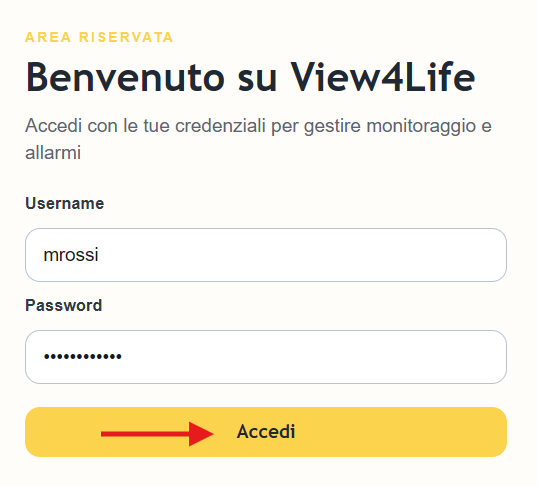
\includegraphics[width=0.5\textwidth]{./img/accesso.png}
            \caption{Schermata di accesso}
        \end{figure}
\end{enumerate}

\subsection{Collegare l'utente Amministratore al relativo \textit{account MyVimar}}
\begin{enumerate}
    \item Dal menu principale, selezionare la voce \textbf{Profilo};
        \begin{figure}[H]
            \centering
            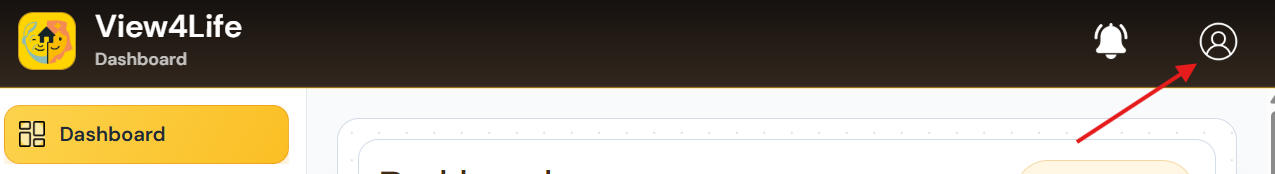
\includegraphics[width=0.6\textwidth]{./img/clicca_profilo.png}
            \caption{Voce Profilo nel menu principale}
        \end{figure}
    \item Premere \textbf{Vai a MyVimar};
        \begin{figure}[H]
            \centering
            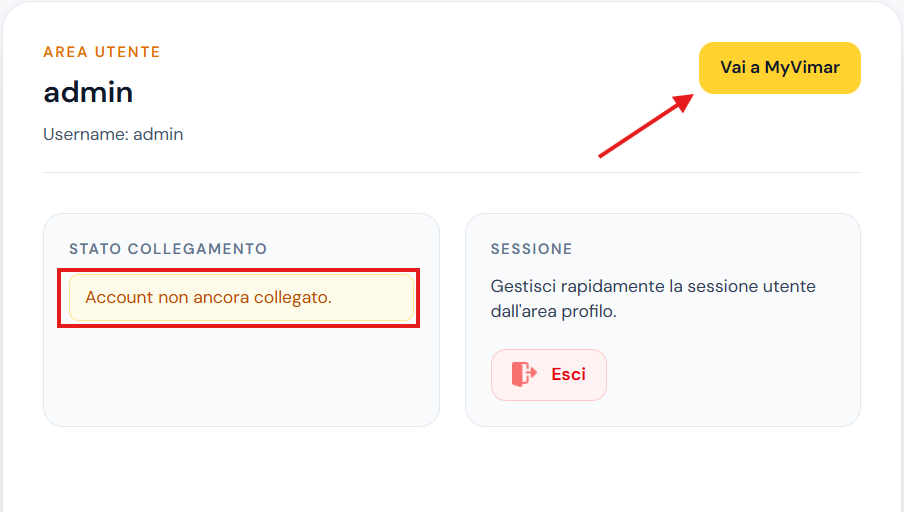
\includegraphics[width=0.8\textwidth]{./img/vai_myvimar.png}
            \caption{Pulsante Vai a MyVimar nella schermata Profilo}
        \end{figure}
    \item Premere su \textbf{Collega account MyVimar};
        \begin{figure}[H]
            \centering
            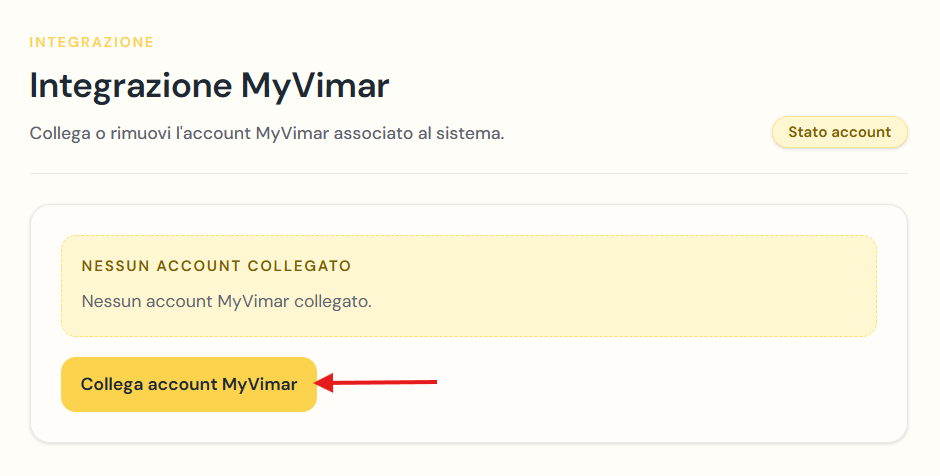
\includegraphics[width=0.6\textwidth]{./img/collega_account_myvari.png}
            \caption{Pulsante Collega account MyVimar}
        \end{figure}
    \item Il Sistema reindirizza al portale di autenticazione di Vimar;
        \begin{figure}[H]
            \centering
            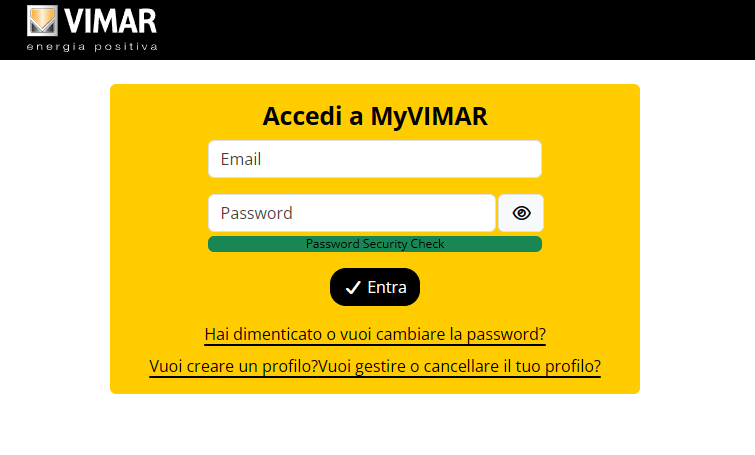
\includegraphics[width=0.5\textwidth]{./img/pagina_gialla_vimar.png}
            \caption{Portale di autenticazione Vimar}
        \end{figure}
    \item Inserire le credenziali MyVimar e premere \textbf{Entra};
    \item Il Sistema registra il collegamento e mostra l'indirizzo email 
          dell'account MyVimar collegato.
        \begin{figure}[H]
            \centering
            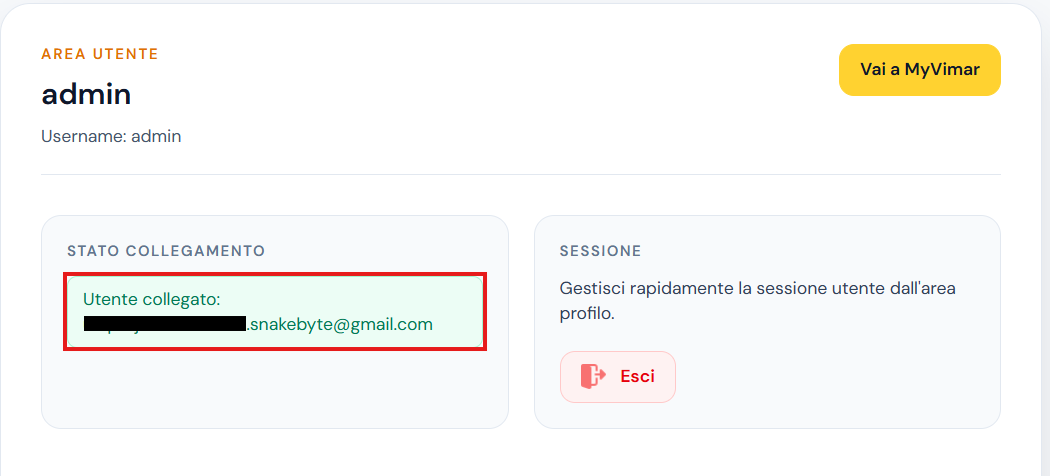
\includegraphics[width=0.8\textwidth]{./img/stato_collegamento_myVimar.png}
            \caption{Stato del collegamento all'account MyVimar}
        \end{figure}
\end{enumerate}

\subsection{Scollegare l'utente Amministratore dal relativo \textit{account MyVimar}}
\begin{enumerate}
    \item Dal menu principale, selezionare la voce \textbf{Profilo};
    \item Premere \textbf{Vai a MyVimar};

    \begin{figure}[H]
        \centering
        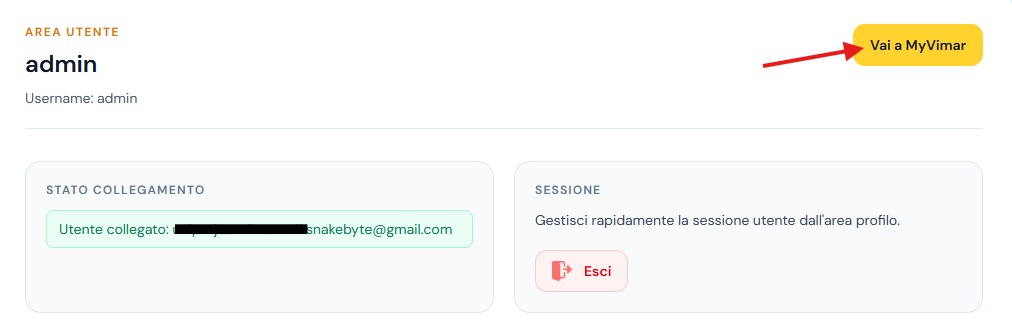
\includegraphics[width=0.8\textwidth]{img/bottone_myvimar.png}
        \caption{Pulsante Vai a MyVimar nella schermata Profilo}
    \end{figure}

    \item Premere il pulsante \textbf{Rimuovi account};

    \begin{figure}[H]
        \centering
        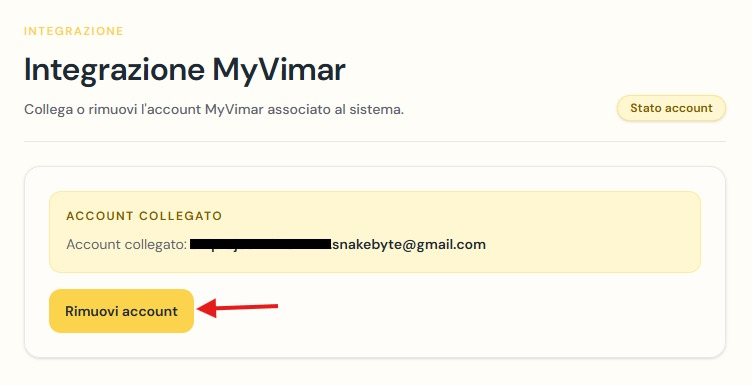
\includegraphics[width=0.8\textwidth]{img/pulsante_rimuovi_account.png}
        \caption{Pulsante Rimuovi account nella schermata Integrazione MyVimar}
    \end{figure}

    \item Il Sistema rimuove il collegamento e mostra la schermata 
    con nessun account collegato.

    \begin{figure}[H]
        \centering
        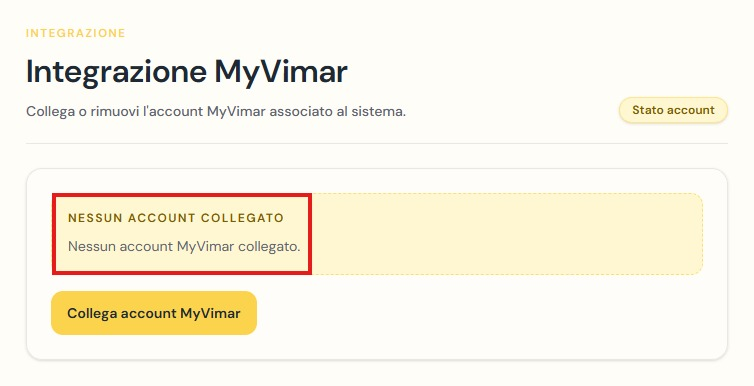
\includegraphics[width=0.8\textwidth]{img/account_scollegato.png}
        \caption{Schermata Integrazione MyVimar dopo la rimozione dell'account}
    \end{figure}

\end{enumerate}


\subsection{Visualizzare la \textit{Dashboard}}
\begin{enumerate}
    \item Dal menu principale, selezionare la voce \textit{\textbf{Dashboard}};
        \begin{figure}[H]
            \centering
            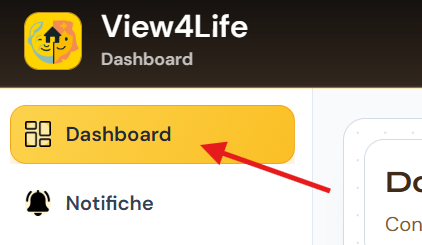
\includegraphics[width=0.4\textwidth]{./img/vai_dashboard.png}
            \caption{Voce Dashboard nel menu principale}
        \end{figure}
    \item Il Sistema mostra la \textit{Dashboard}, che include sempre il modulo
          \textbf{Gestione Allarmi} e i seguenti moduli:
          \begin{itemize}
              \item Statistiche Allarmi;
              \item Analisi Consumi;
              \item Struttura appartamento.
          \end{itemize}
        \begin{figure}[H]
            \centering
            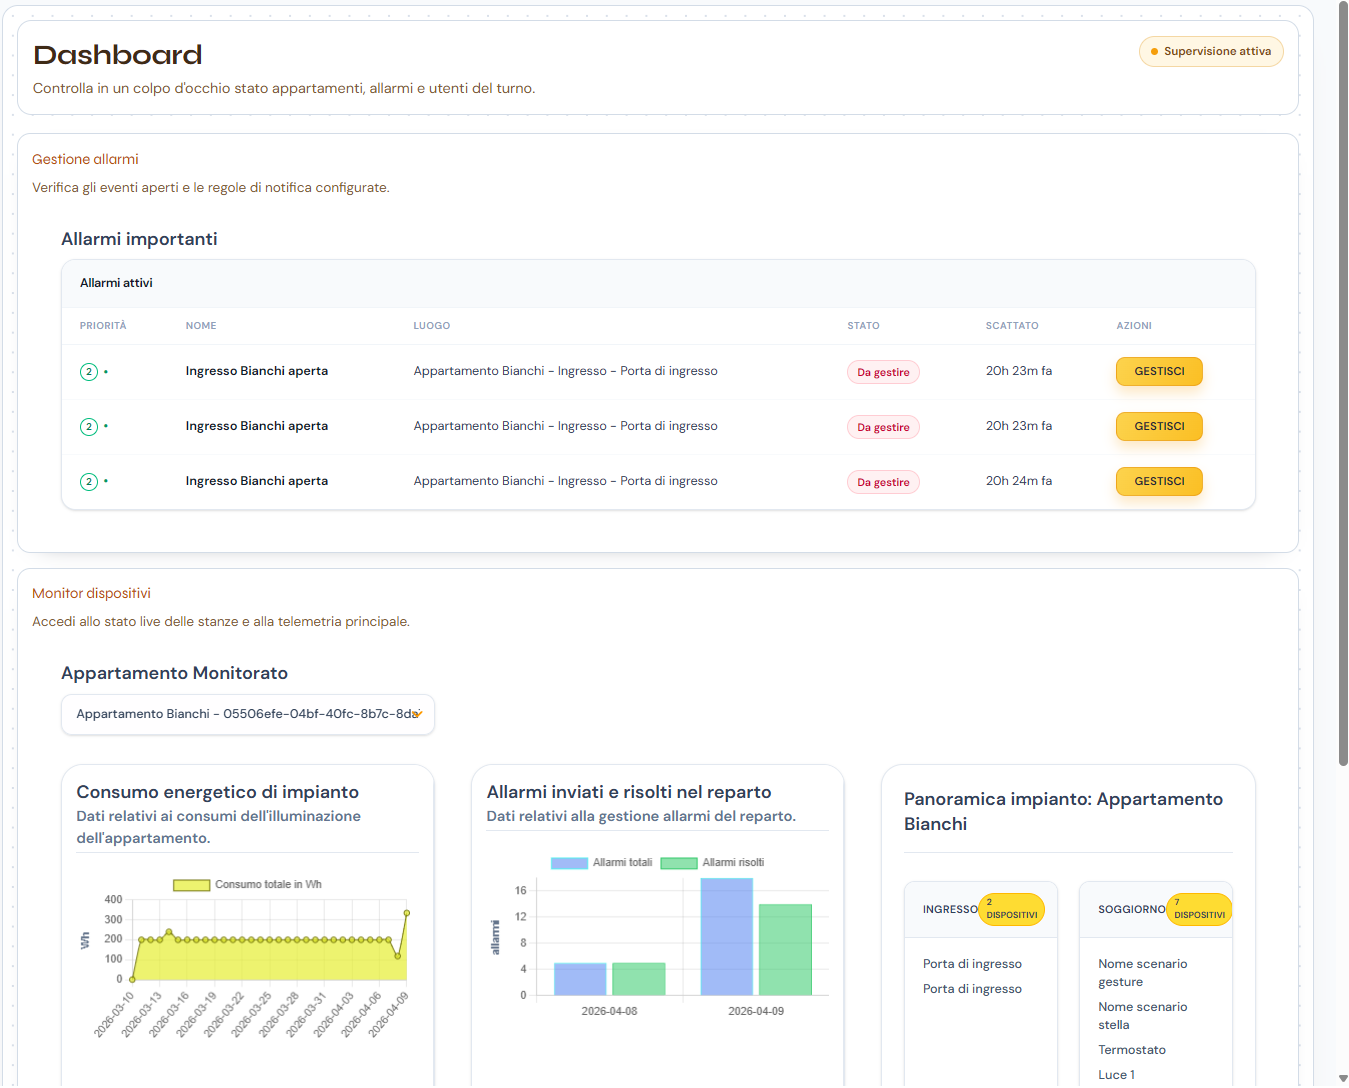
\includegraphics[width=\textwidth]{./img/dashboard.png}
            \caption{Schermata principale della Dashboard}
        \end{figure}
\end{enumerate}

\subsection{Gestire le notifiche}
\subsubsection{Visualizzare le notifiche}
\begin{enumerate}
    \item Dal menu principale, selezionare la voce \textbf{Notifiche}.
        \begin{figure}[H]
            \centering
            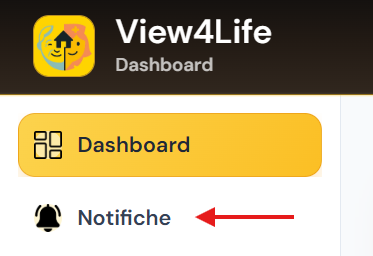
\includegraphics[width=0.4\textwidth]{./img/voce_notifiche.png}
            \caption{Voce Notifiche nel menu principale}
        \end{figure}
    \item Il Sistema mostra l'elenco delle notifiche. Per ogni notifica sono visibili:
          \begin{itemize}
              \item Il \textbf{titolo} della notifica;
              \item il \textbf{tempo trascorso} dall'invio.
          \end{itemize}
        \begin{figure}[H]
            \centering
            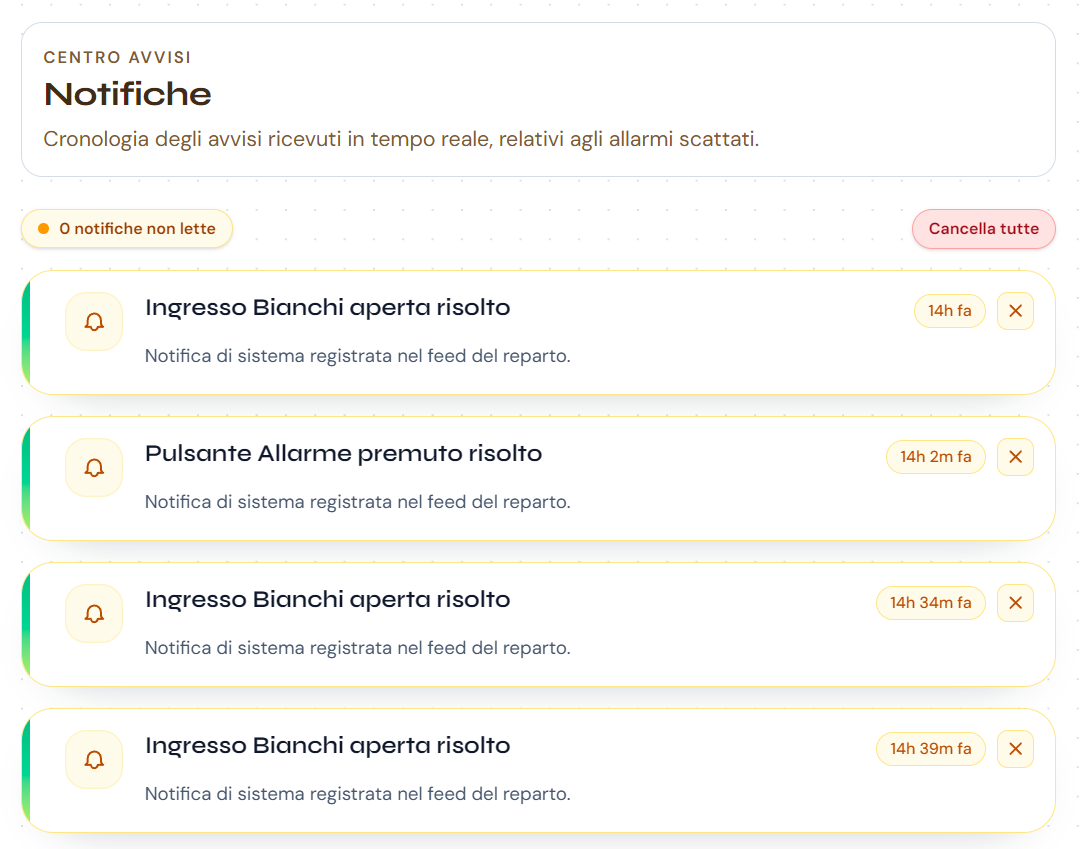
\includegraphics[width=0.8\textwidth]{./img/elenco_notifiche.png}
            \caption{Elenco delle notifiche}
        \end{figure}
\end{enumerate}

\subsubsection{Eliminare le notifiche}
\begin{enumerate}
    \item Dal menu principale, selezionare la voce \textbf{Notifiche};
    \item Individuare la notifica da eliminare nell'elenco;
    \item Premere il pulsante \textbf{Elimina} accanto alla notifica;
        \begin{figure}[H]
            \centering
            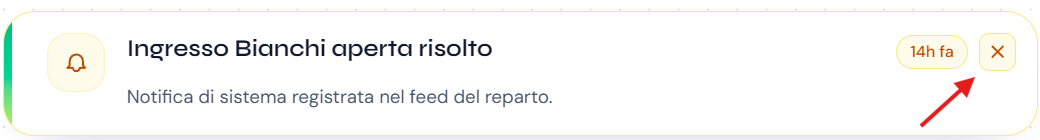
\includegraphics[width=0.7\textwidth]{./img/elimina_notifica.png}
            \caption{Pulsante Elimina per una singola notifica}
        \end{figure}
    \item Se si vogliono eliminare tutte le notifiche, premere il pulsante \textbf{Cancella tutte};
        \begin{figure}[H]
            \centering
            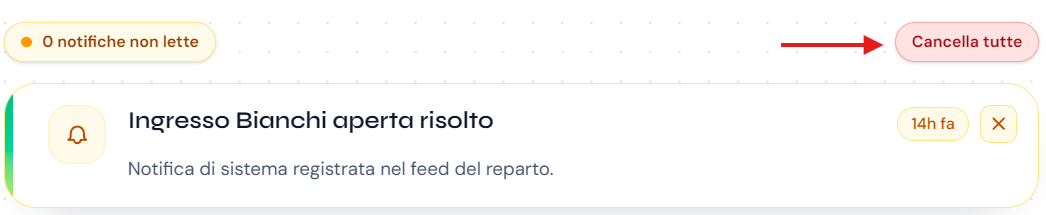
\includegraphics[width=0.7\textwidth]{./img/elimina_tutte_notifiche.png}
            \caption{Pulsante Cancella tutte le notifiche}
        \end{figure}
    \item Il Sistema rimuove la notifica dall'elenco.
\end{enumerate}

\subsection{Gestire i dispositivi di un appartamento}
\subsubsection{Visualizzare i dispositivi}
\begin{enumerate}
    \item Dal menu principale, selezionare la voce \textbf{Dispositivi};
        \begin{figure}[H]
            \centering
            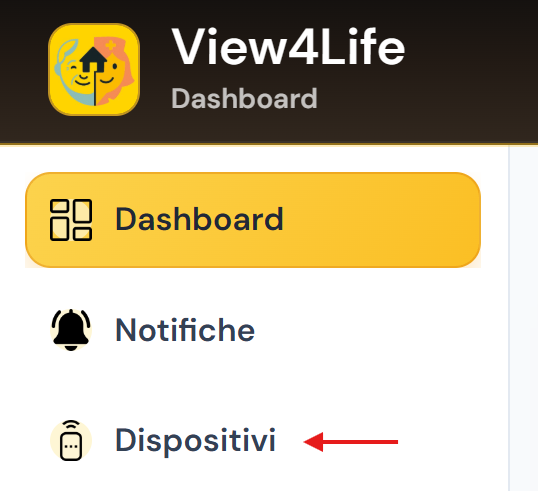
\includegraphics[width=0.4\textwidth]{./img/voce_dispositivi.png}
            \caption{Voce Dispositivi nel menu principale}
        \end{figure}
    \item Selezionare l'appartamento desiderato;
        \begin{figure}[H]
            \centering
            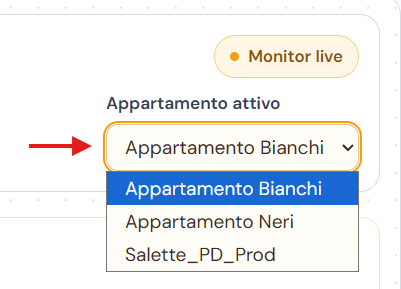
\includegraphics[width=0.4\textwidth]{./img/selettore_appartamento_dispositivi.png}
            \caption{Selettore appartamento nella sezione Dispositivi}
        \end{figure}
    \item Il Sistema mostra la vista dell'appartamento, con l'elenco delle stanze; 
    \item Il Sistema mostra l'elenco dei dispositivi suddivisi per stanza.\\
          Per ogni dispositivo sono visibili:
          \begin{itemize}
              \item Il \textbf{nome} del dispositivo;
              \item Il \textbf{tipo};
              \item L'\textbf{endpoint} associato;
              \item lo \textbf{stato} attuale;
              \item un selettore di \textbf{valore};
              \item l' \textbf{azione} di scrittura.
          \end{itemize}
        \begin{figure}[H]
            \centering
            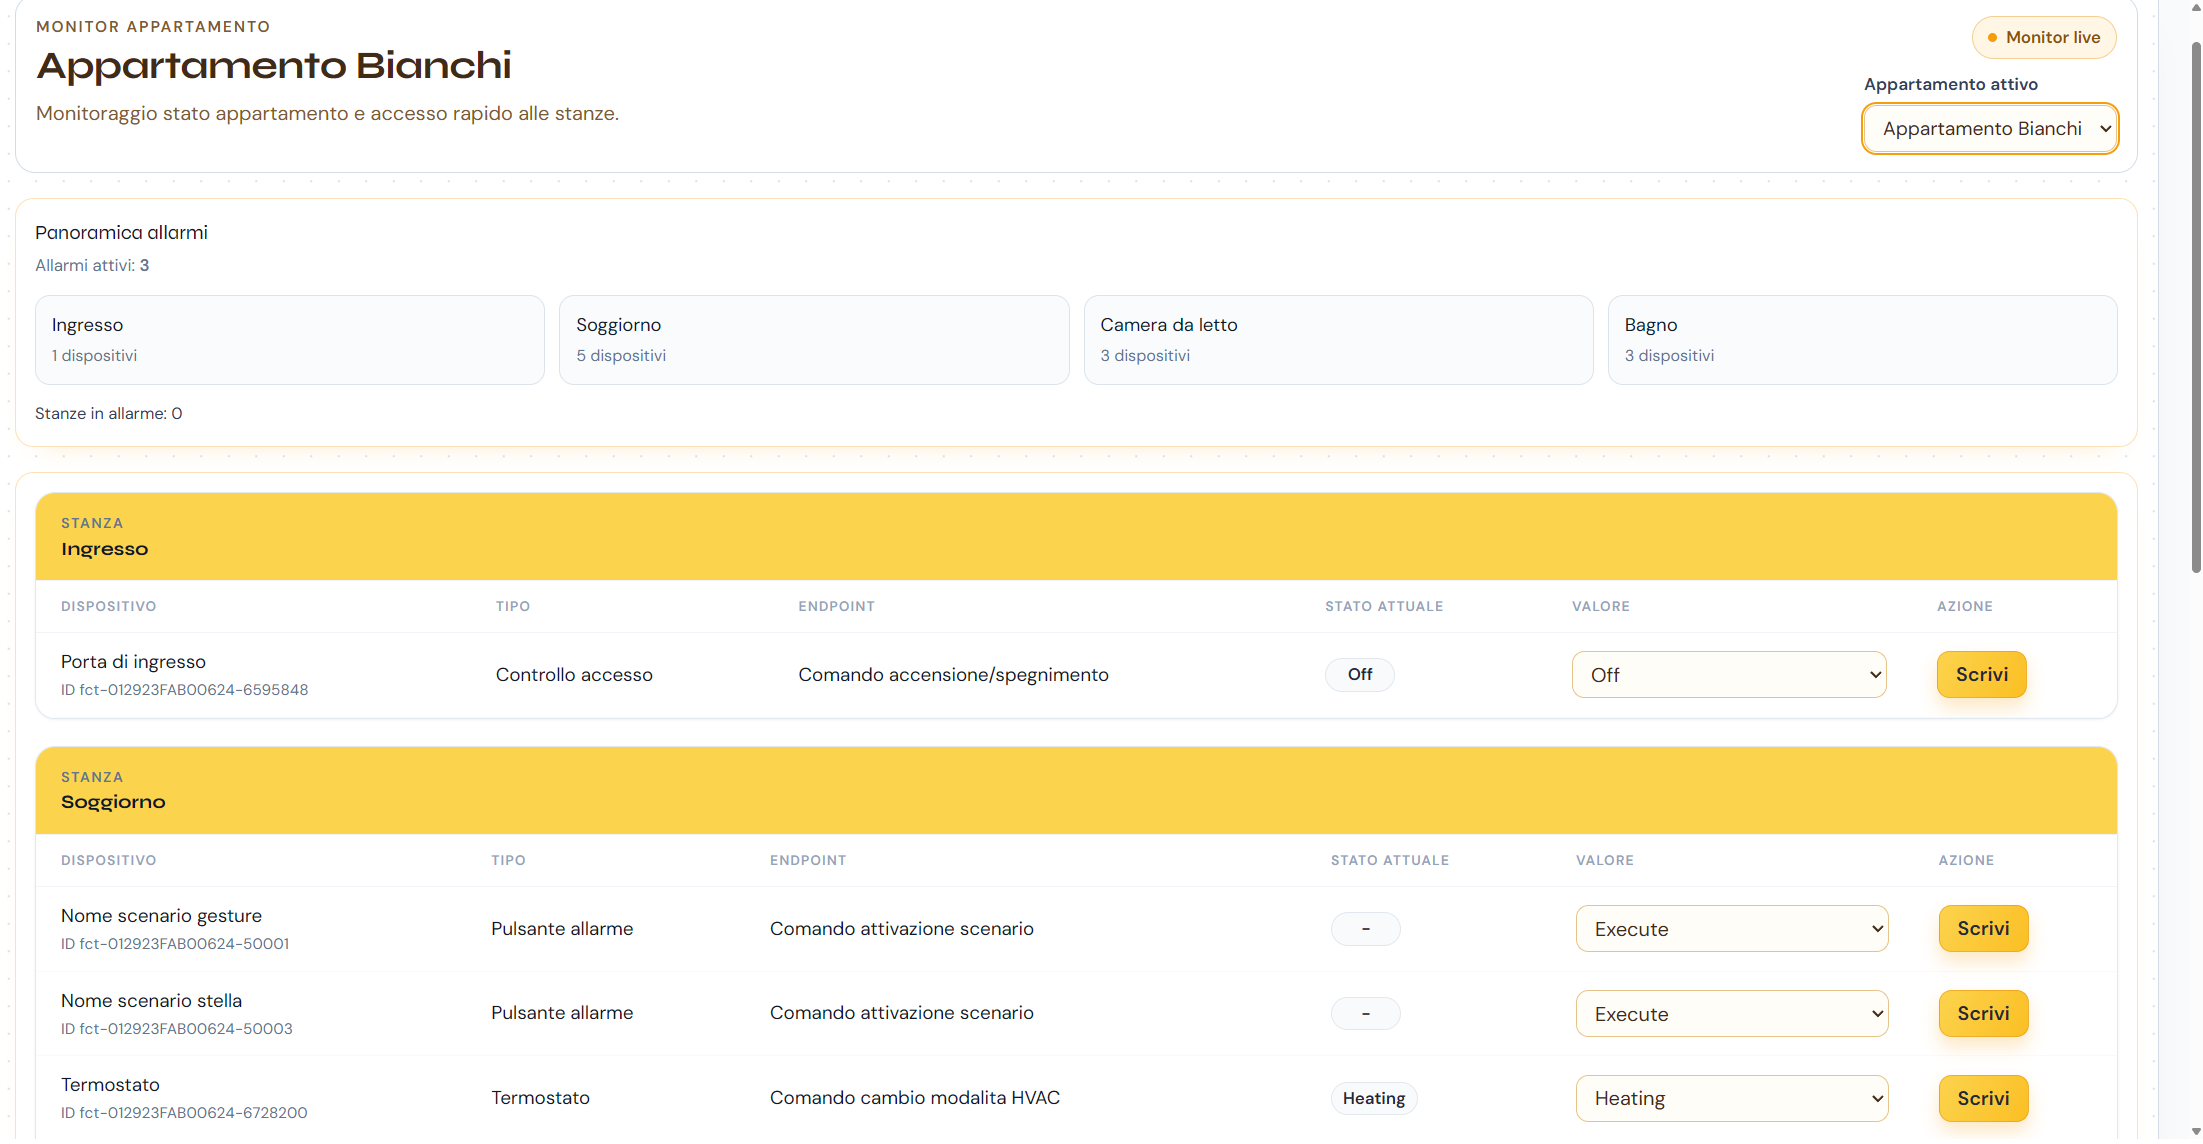
\includegraphics[width=\textwidth]{./img/elenco_dispositivi.png}
            \caption{Elenco dei dispositivi suddivisi per stanza}
        \end{figure}
\end{enumerate}

\subsubsection{Modificare lo stato dei dispositivi}
\begin{enumerate}
    \item Visualizzare i dispositivi della stanza seguendo i passi descritti 
          nella sezione precedente;
    \item Individuare il dispositivo da modificare;
    \item Selezionare l'azione desiderata tra quelle disponibili per il dispositivo;
        \begin{figure}[H]
            \centering
            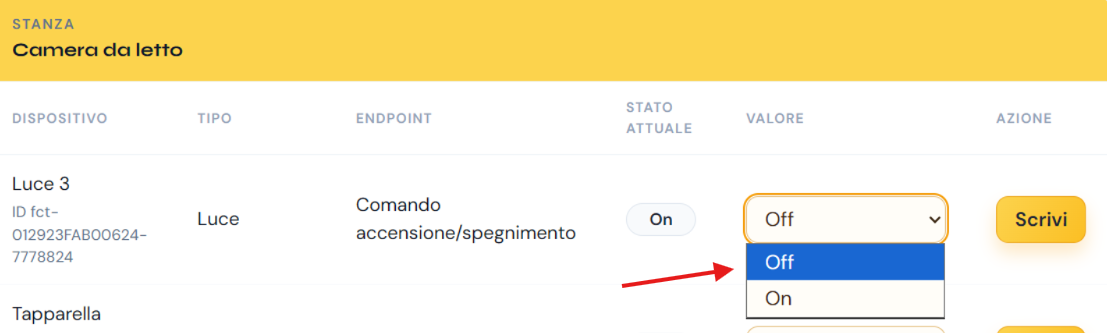
\includegraphics[width=\textwidth]{./img/opzioni_disp.png}
            \caption{Opzioni disponibili per la modifica di un dispositivo}
        \end{figure}
    \item Dopo aver selezionato il nuovo stato, premere \textbf{Scrivi};
        \begin{figure}[H]
            \centering
            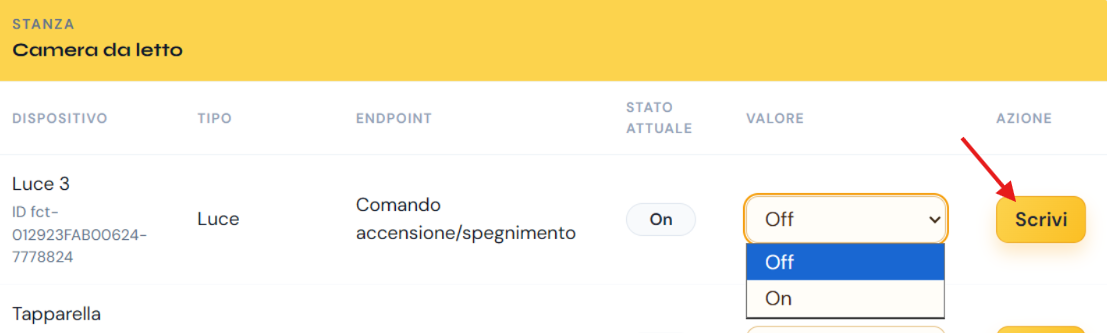
\includegraphics[width=\textwidth]{./img/scrivi.png}
            \caption{Pulsante Scrivi per confermare la modifica del dispositivo}
        \end{figure}
    \item Il Sistema invia il comando al dispositivo e comunica all'utente il cambio di stato;
        \begin{figure}[H]
            \centering
            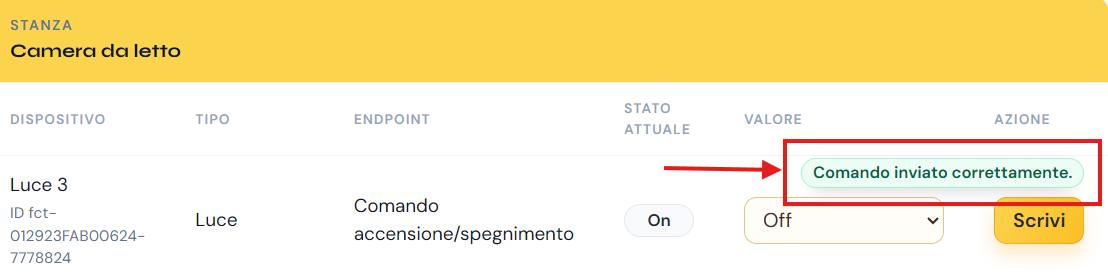
\includegraphics[width=\textwidth]{./img/comando_corr.png}
            \caption{Conferma dell'avvenuto cambio di stato del dispositivo}
        \end{figure}
    \item Per poter visualizzare il nuovo stato del dispositivo è necessario ricaricare la pagina.
\end{enumerate}

\subsection{Gestire gli allarmi attivi}
\subsubsection{Visualizzare gli allarmi attivi}
Il modulo \textbf{Gestione Allarmi} è sempre visibile nella Dashboard e dalla voce del menu principale \textbf{Gestione Allarmi} e presenta
l'elenco degli allarmi correntemente attivi. Per ogni allarme sono mostrati:
\begin{itemize}
    \item Il \textbf{segnale di pericolo} (indicatore visivo del livello di priorità);
    \item il \textbf{nome} dell'allarme;
    \item il \textbf{luogo} in cui è scattato l'allarme;
    \item il \textbf{tempo trascorso} dallo scatto dell'allarme.
\end{itemize}
\begin{figure}[H]
    \centering
    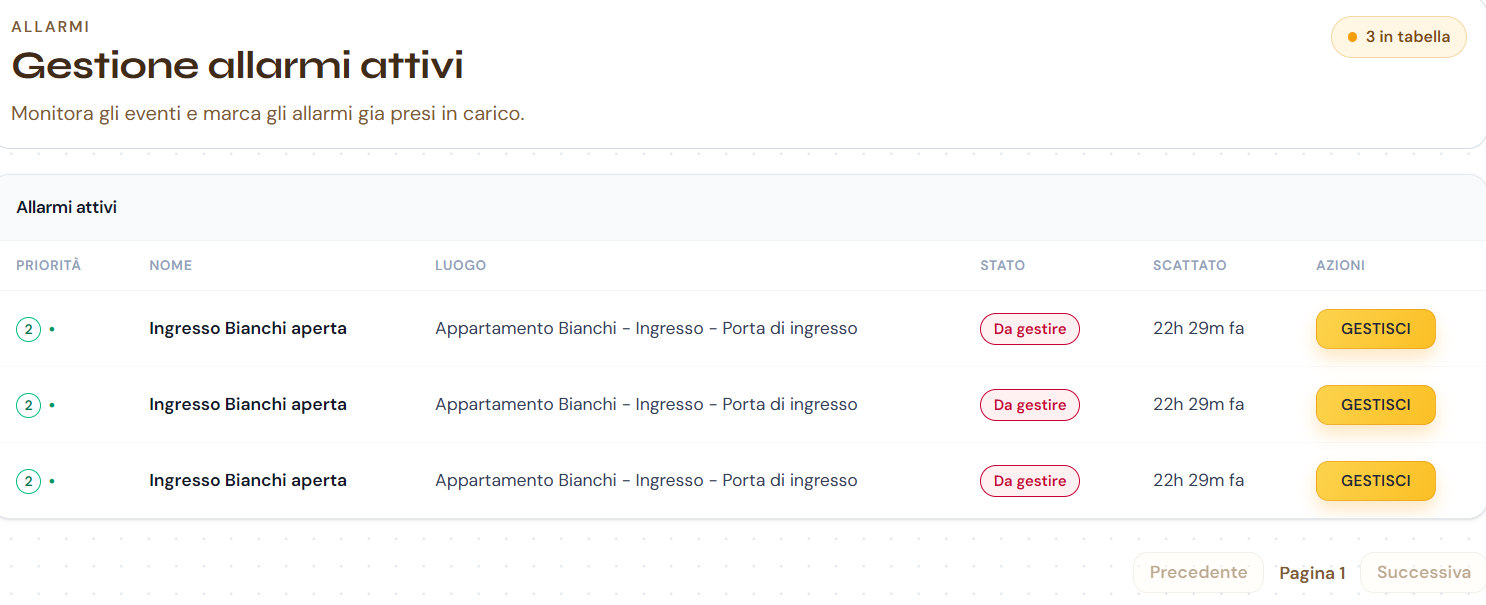
\includegraphics[width=\textwidth]{./img/gestione-allarmi.png}
    \caption{Modulo Gestione Allarmi con elenco degli allarmi attivi}
\end{figure}

\subsubsection{Risolvere un allarme attivo}
\begin{enumerate}
    \item Dal menu principale, selezionare la voce \textbf{Gestione Allarmi};
    \item Individuare l'allarme da risolvere;
    \item Premere il pulsante \textbf{Gestisci} accanto all'allarme;
        \begin{figure}[H]
            \centering
            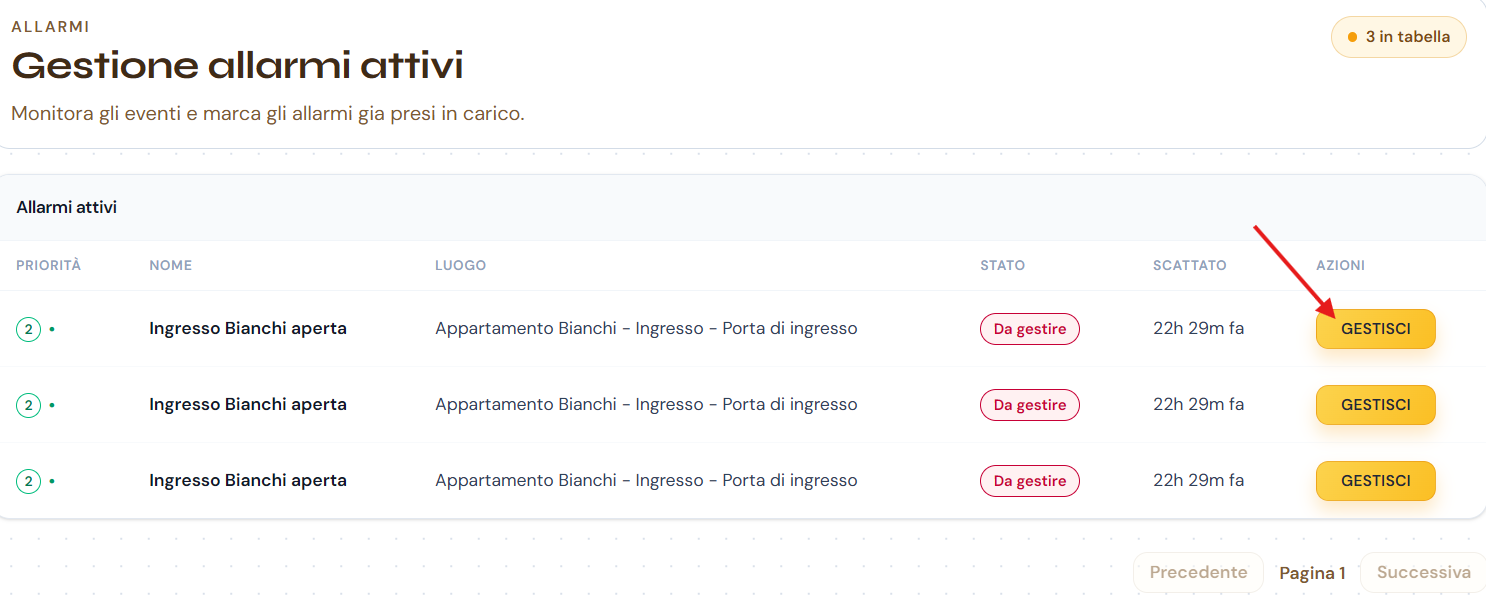
\includegraphics[width=\textwidth]{./img/gestisci.png}
            \caption{Pulsante Gestisci per la risoluzione di un allarme}
        \end{figure}
    \item Il Sistema contrassegna l'allarme come risolto e lo rimuove dall'elenco degli allarmi attivi.
\end{enumerate}

\subsubsection{Visualizzare lo storico degli allarmi risolti}
\begin{enumerate}
    \item Dal menu principale, selezionare la voce \textbf{Storico Allarmi};
        \begin{figure}[H]
            \centering
            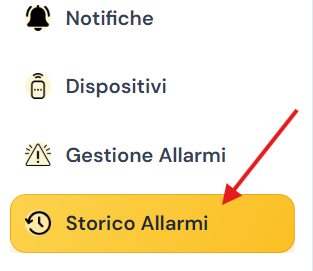
\includegraphics[width=0.4\textwidth]{./img/voce_storico_allarmi.png}
            \caption{Voce Storico Allarmi nel menu principale}
        \end{figure}
    \item Il Sistema mostra l'elenco degli allarmi contrassegnati come risolti. 
          Per ogni allarme sono visibili:
          \begin{itemize}
              \item Il \textbf{nome} dell'allarme;
              \item il \textbf{luogo} in cui è scattato;
              \item l' \textbf{orario di scatto};
              \item l' \textbf{orario di risoluzione};
              \item il \textbf{gestore} dell'allarme.
          \end{itemize}
        \begin{figure}[H]
            \centering
            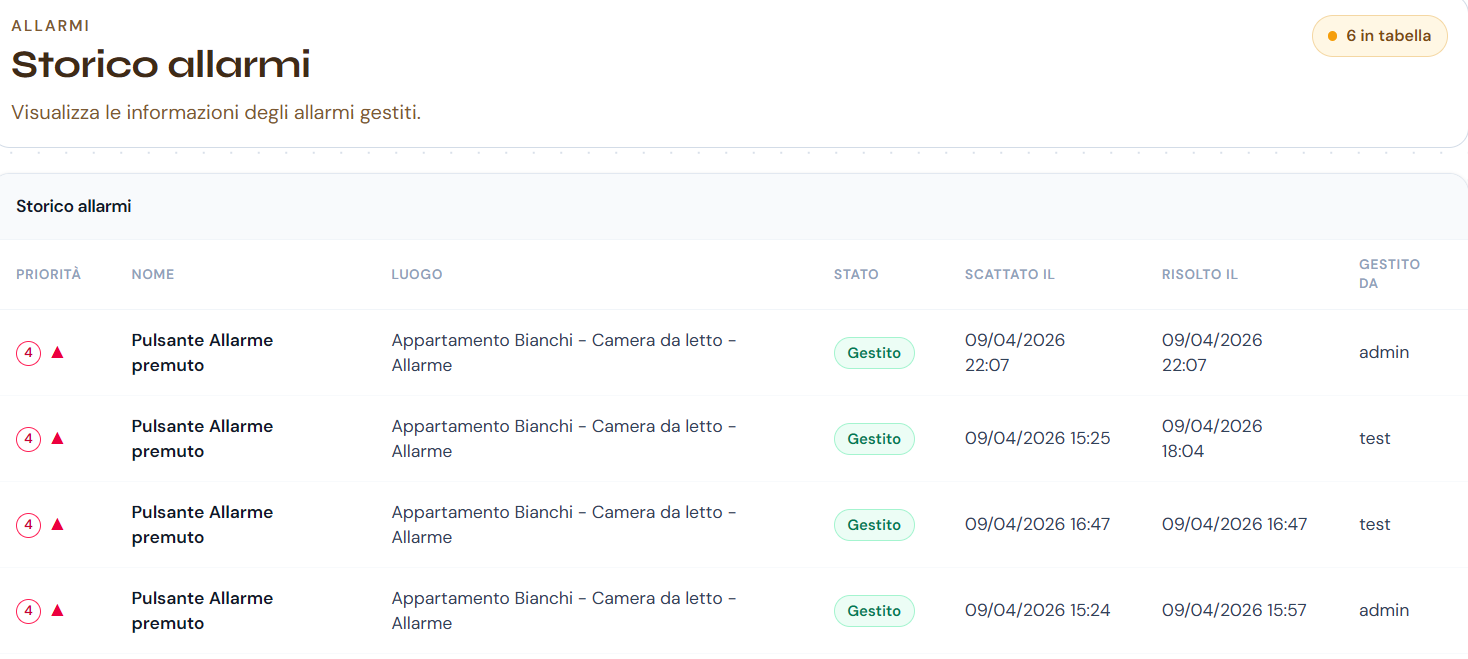
\includegraphics[width=\textwidth]{./img/storico_allarmi.png}
            \caption{Schermata Storico degli allarmi risolti}
        \end{figure}
\end{enumerate}

\subsection{Gestire le regole di allarme}
La configurazione degli allarmi è riservata all'\admin. Ogni allarme è associato
al \textit{datapoint} di un dispositivo di un appartamento e definisce la condizione 
che scatena un allarme e la relativa notifica agli utenti associati al reparto corrispondente.
\\I parametri configurabili per ogni allarme sono:
\begin{itemize}
    \item \textbf{Nome} dell'allarme;
    \item \textbf{Appartamento} a cui l'allarme è associato;
    \item \textbf{Dispositivo} e relativo \textit{\textbf{Datapoint}} che scatena l'allarme;
    \item \textbf{Livello di priorità}, scelto tra quattro livelli:
          \begin{itemize}
              \item Livello 1: Bianco (priorità minima);
              \item Livello 2: Verde;
              \item Livello 3: Arancione;
              \item Livello 4: Rosso (priorità massima).
          \end{itemize}
    \item \textbf{Soglia di intervento}: condizione che fa scattare l'allarme;
    \item \textbf{Orario di attivazione}: orario a partire dal quale l'allarme è operativo;
    \item \textbf{Orario di disattivazione}: orario a partire dal quale l'allarme viene sospeso.
\end{itemize}

\subsubsection{Creare una nuova regola di allarme}
\begin{enumerate}
    \item Dal menu principale, selezionare la voce \textbf{Configurazione Allarmi};
        \begin{figure}[H]
            \centering
            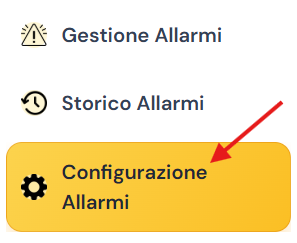
\includegraphics[width=0.4\textwidth]{./img/config_allarmi.png}
            \caption{Voce Configurazione Allarmi nel menu principale}
        \end{figure}
    \item Premere il pulsante '+' (\textbf{Nuovo allarme});
        \begin{figure}[H]
            \centering
            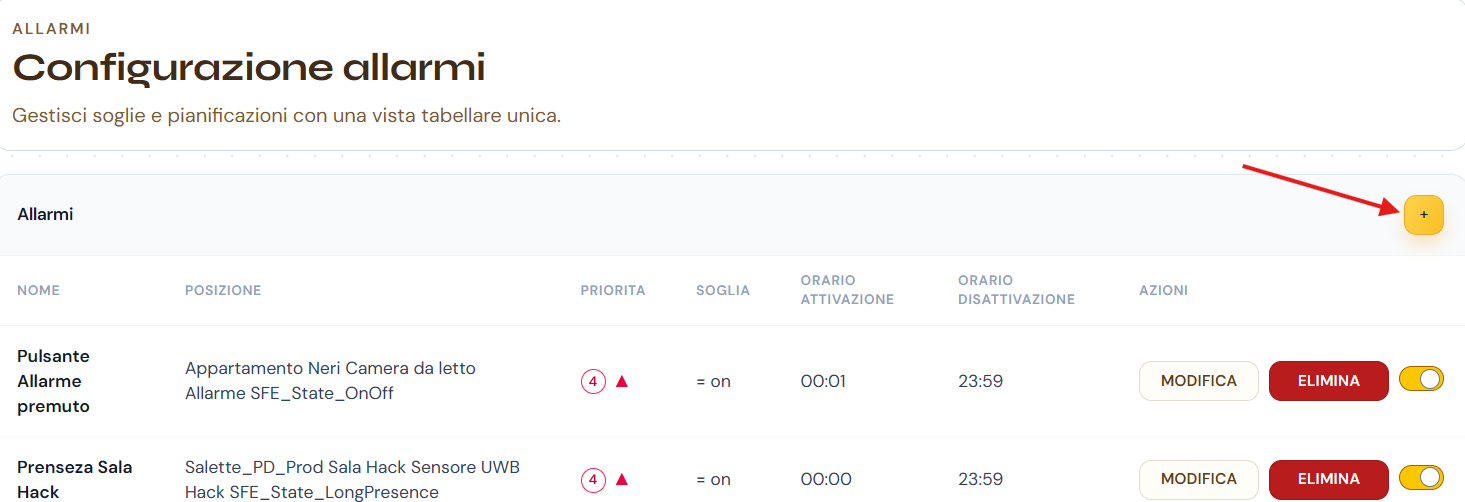
\includegraphics[width=\textwidth]{./img/nuova_regola_allarme.png}
            \caption{Pulsante Nuovo allarme nella sezione Configurazione Allarmi}
        \end{figure}
    \item Compilare il \textbf{form} della nuova regola di allarme;\\
    "\textbf{NOTA}: i campi \textbf{Nome}, \textbf{Appartamento}, \textbf{Dispositivo} e \textbf{Datapoint} non saranno modificabili dopo la creazione della regola. In caso di errore sarà necessario eliminare la regola e crearne una nuova."
        \begin{figure}[H]
            \centering
            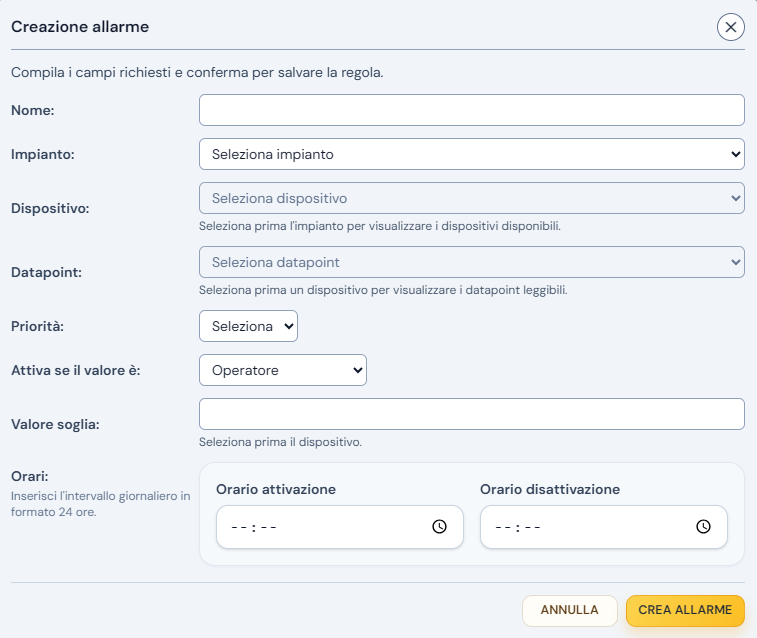
\includegraphics[width=0.8\textwidth]{./img/form_allarme.png}
            \caption{Form di creazione di una nuova regola di allarme}
        \end{figure}
    \item Compilare tutti i campi richiesti. 
    Infine premere \textbf{Crea Allarme} per confermare. Il Sistema salva l'allarme e lo aggiunge
          all'elenco.
        \begin{figure}[H]
            \centering
            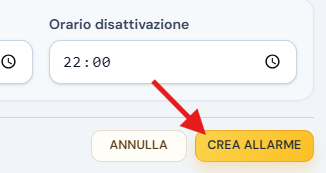
\includegraphics[width=0.4\textwidth]{./img/crea_allarme.png}
            \caption{Pulsante Crea Allarme per confermare la nuova regola}
        \end{figure}
\end{enumerate}

\subsubsection{Abilitare una regola di allarme}
\begin{enumerate}
    \item Dalla sezione \textbf{Configurazione Allarmi}, individuare l'allarme da abilitare.
    \item Premere il pulsante di commutazione corrispondente.
        \begin{figure}[H]
            \centering
            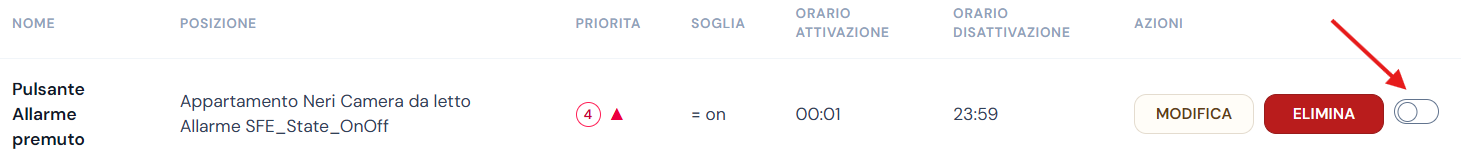
\includegraphics[width=\textwidth]{./img/abilitare_allame.png}
            \caption{Pulsante di commutazione per abilitare una regola di allarme}
        \end{figure}
    \item Il Sistema attiva l'allarme: da questo momento il \textit{datapoint} associato può scatenarlo.
\end{enumerate}

\subsubsection{Disabilitare una regola di allarme}
\begin{enumerate}
    \item Dalla sezione \textbf{Configurazione Allarmi}, individuare l'allarme da disabilitare.
    \item Premere il pulsante di commutazione corrispondente.
        \begin{figure}[H]
            \centering
            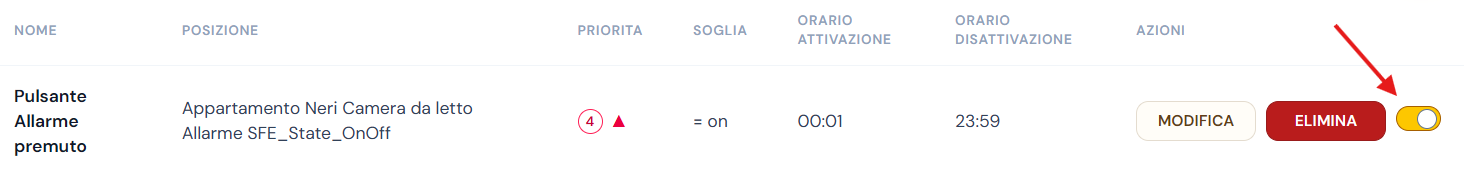
\includegraphics[width=\textwidth]{./img/disabilitare_allarme.png}
            \caption{Pulsante di commutazione per disabilitare una regola di allarme}
        \end{figure}
    \item Il Sistema disattiva l'allarme: da questo momento il \textit{datapoint} associato non può scatenarlo.
\end{enumerate}

\subsubsection{Visualizzare le regole di allarme}
\begin{enumerate}
    \item Dal menu principale, selezionare la voce \textbf{Configurazione Allarmi};
    \item Il Sistema mostra l'elenco delle regole di allarme configurate. 
          Per ogni regola sono visibili:
          \begin{itemize}
              \item Il \textbf{nome} dell'allarme;
              \item la \textbf{posizione} del dispositivo associato;
              \item il \textbf{livello di priorità};
              \item il \textbf{valore di soglia};
              \item l'\textbf{orario di attivazione};
              \item l'\textbf{orario di disattivazione};
              \item lo \textbf{stato} (abilitato/disabilitato).
          \end{itemize}
        \begin{figure}[H]
            \centering
            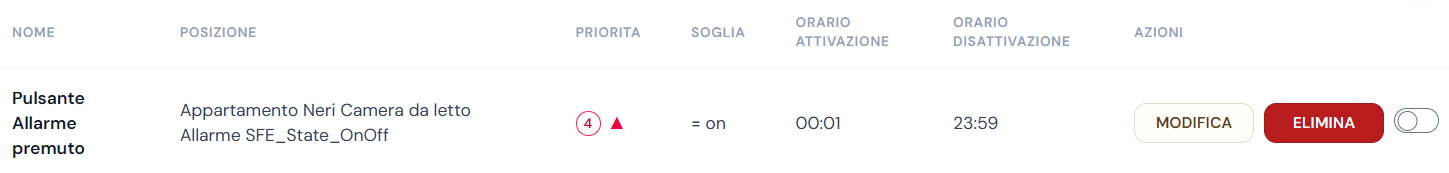
\includegraphics[width=\textwidth]{./img/caratt_regole.png}
            \caption{Elenco delle regole di allarme configurate con le relative caratteristiche}
        \end{figure}
\end{enumerate}

\subsubsection{Modificare una regola di allarme}
L'\admin può modificare singolarmente i parametri di un allarme esistente.
Gli unici parametri modificabili sono: priorità, valore di soglia e orari di attivazione/disattivazione.

\paragraph{Modificare la priorità}
\begin{enumerate}
    \item Dalla sezione \textbf{Configurazione Allarmi}, selezionare l'allarme da modificare premendo su \textbf{Modifica};
    \item Selezionare il campo \textbf{Priorità};
        \begin{figure}[H]
            \centering
            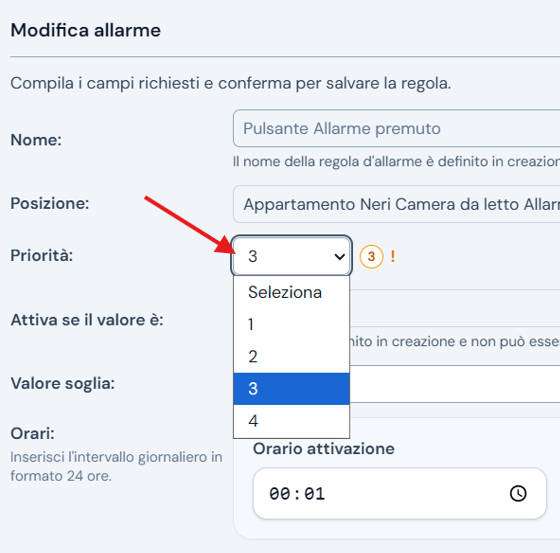
\includegraphics[width=0.6\textwidth]{./img/modifica_priorita.png}
            \caption{Campo Priorità nel form di modifica della regola di allarme}
        \end{figure}
    \item Selezionare il nuovo livello di priorità e premere il bottone \textbf{Applica modifiche}.
\end{enumerate}

\paragraph{Modificare la soglia di intervento}
\begin{enumerate}
    \item Dalla sezione \textbf{Configurazione Allarmi}, selezionare l'allarme da modificare premendo su \textbf{Modifica};
    \item Selezionare il campo \textbf{Valore soglia};
        \begin{figure}[H]
            \centering
            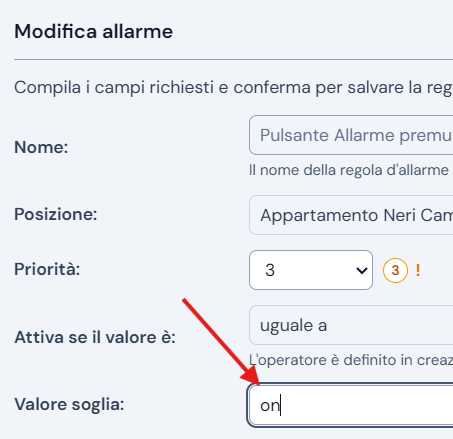
\includegraphics[width=0.6\textwidth]{./img/modifica_soglia.png}
            \caption{Campo Valore soglia nel form di modifica della regola di allarme}
        \end{figure}
    \item Selezionare il nuovo valore di soglia e premere il bottone \textbf{Applica modifiche}.
\end{enumerate}

\paragraph{Modificare gli orari}
\begin{enumerate}
    \item Dalla sezione \textbf{Configurazione Allarmi}, selezionare l'allarme da modificare premendo su \textbf{Modifica}.
    \item Selezionare il campo \textbf{Orari};
        \begin{figure}[H]
            \centering
            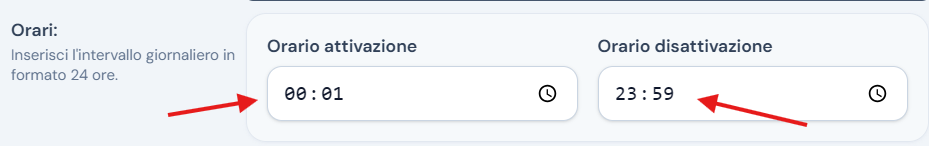
\includegraphics[width=0.8\textwidth]{./img/modifica_orario.png}
            \caption{Campo Orari nel form di modifica della regola di allarme}
        \end{figure}
    \item Inserire il nuovo orario e premere il bottone \textbf{Applica modifiche}.
\end{enumerate}

\subsubsection{Eliminare una regola di allarme}
\begin{enumerate}
    \item Dalla sezione \textbf{Configurazione Allarmi}, selezionare l'allarme da eliminare premendo su \textbf{Elimina};
        \begin{figure}[H]
            \centering
            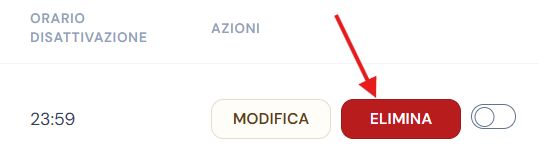
\includegraphics[width=0.4\textwidth]{./img/elimina_allarme.png}
            \caption{Pulsante Elimina per una regola di allarme}
        \end{figure}
    \item Confermare nuovamente l'eliminazione premendo sul bottone \textbf{Elimina}.
        \begin{figure}[H]
            \centering
            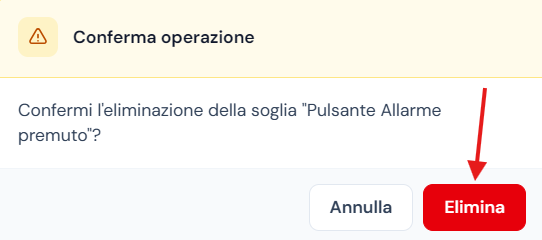
\includegraphics[width=0.4\textwidth]{./img/elimina_allarme_conferma.png}
            \caption{Dialogo di conferma eliminazione della regola di allarme}
        \end{figure}
\end{enumerate}

\subsection{Visualizzare le \textit{Analytics} di un appartamento}
\begin{enumerate}
    \item Dal menu principale, selezionare la voce \textbf{Analytics};
        \begin{figure}[H]
            \centering
            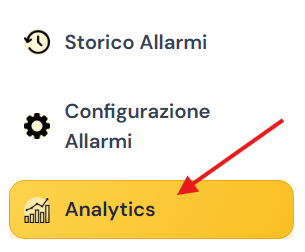
\includegraphics[width=0.4\textwidth]{./img/voce_analytics.png}
            \caption{Voce Analytics nel menu principale}
        \end{figure}
    \item Selezionare l'appartamento di cui si vogliono visualizzare le analytics;
        \begin{figure}[H]
            \centering
            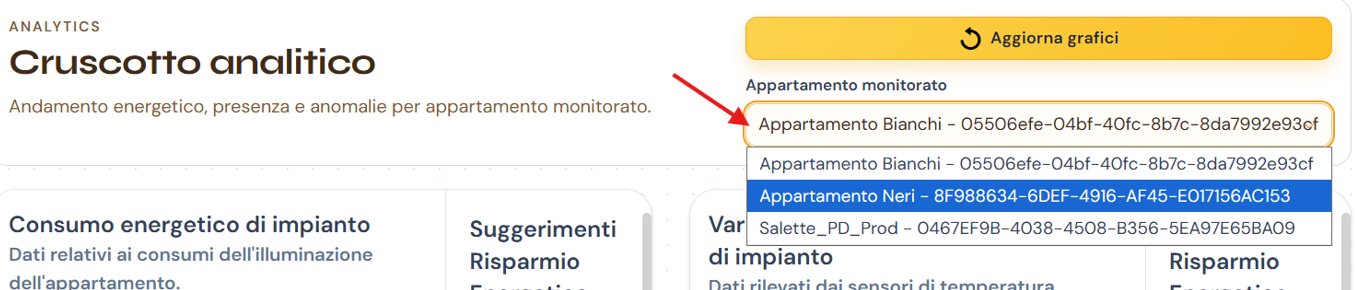
\includegraphics[width=\textwidth]{./img/analytics_sel_app.png}
            \caption{Selettore appartamento nella sezione Analytics}
        \end{figure}
    \item Il Sistema mostra i grafici relativi all'appartamento selezionato, tra cui:
          \begin{itemize}
              \item \textbf{Consumo energetico};
              \item \textbf{Anomalie dell'impianto};
              \item \textbf{Rilevamento di presenza};
              \item \textbf{Presenza prolungata};
              \item \textbf{Variazioni di temperatura};
              \item \textbf{Allarmi inviati e risolti};
              \item \textbf{Frequenza degli allarmi};
              \item \textbf{Frequenza delle cadute}.
          \end{itemize}
        \begin{figure}[H]
            \centering
            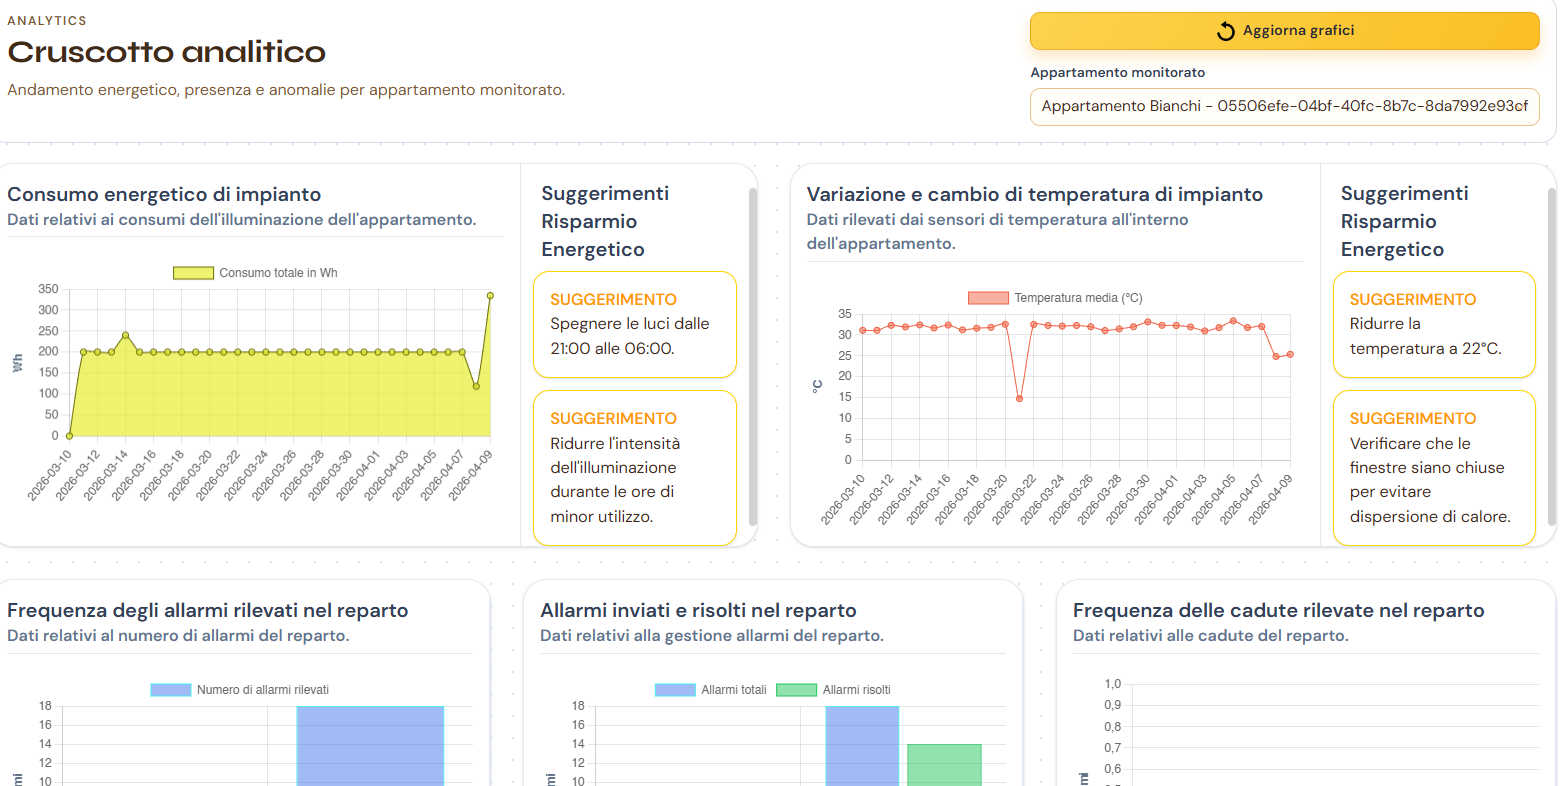
\includegraphics[width=\textwidth]{./img/analytics.png}
            \caption{Schermata Analytics con i grafici dell'appartamento selezionato}
        \end{figure}
\end{enumerate}

\subsection{Gestire i reparti}
\subsubsection{Visualizzare tutti i reparti}
\begin{enumerate}
    \item Dal menu principale, selezionare la voce \textbf{Gestione Reparti};
        \begin{figure}[H]
            \centering
            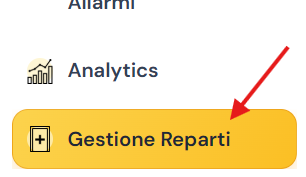
\includegraphics[width=0.4\textwidth]{./img/voce_gestione_rep.png}
            \caption{Voce Gestione Reparti nel menu principale}
        \end{figure}
    \item Il Sistema mostra l'elenco dei reparti configurati. Per ogni reparto 
          sono visibili:
          \begin{itemize}
              \item Il \textbf{nome} del reparto;
              \item l'elenco degli \textbf{appartamenti} associati;
              \item l'elenco degli \textbf{Operatori Sanitari} associati.
          \end{itemize}
        \begin{figure}[H]
            \centering
            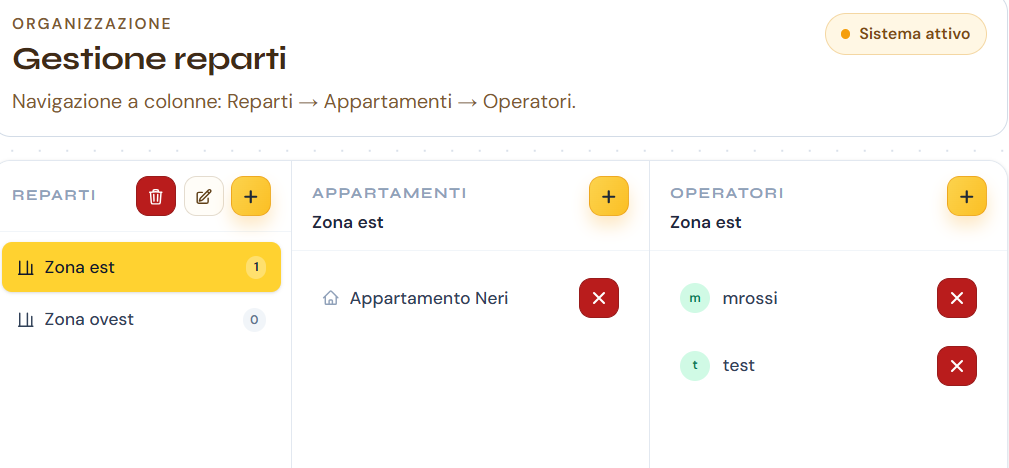
\includegraphics[width=0.8\textwidth]{./img/gestione_rep.png}
            \caption{Schermata Gestione Reparti con l'elenco dei reparti}
        \end{figure}
\end{enumerate}

\subsubsection{Creare un reparto}
\begin{enumerate}
    \item Dalla sezione \textbf{Gestione Reparti}, premere il pulsante '+' \textbf{Nuovo reparto};
        \begin{figure}[H]
            \centering
            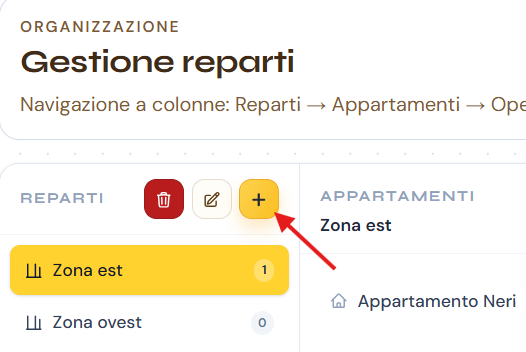
\includegraphics[width=0.5\textwidth]{./img/nuovo_reparto.png}
            \caption{Pulsante Nuovo reparto nella sezione Gestione Reparti}
        \end{figure}
    \item Inserire il \textbf{nome} del reparto e premere \textbf{Crea reparto} per confermare. Il Sistema salva il reparto 
          e lo aggiunge all'elenco.
        \begin{figure}[H]
            \centering
            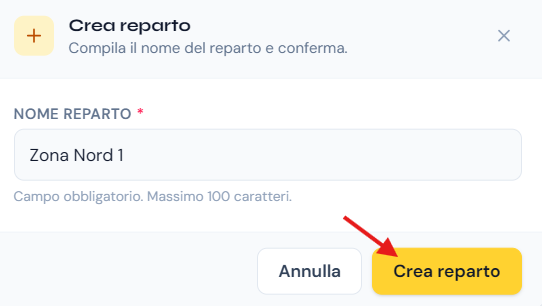
\includegraphics[width=0.5\textwidth]{./img/crea_reparto.png}
            \caption{Form di creazione di un nuovo reparto}
        \end{figure}
\end{enumerate}

\subsubsection{Assegnare un appartamento ad un reparto}
\begin{enumerate}
    \item Dalla sezione \textbf{Gestione Reparti}, selezionare il reparto desiderato;
    \item Selezionare la sezione \textbf{Appartamenti} e premere '+';
        \begin{figure}[H]
            \centering
            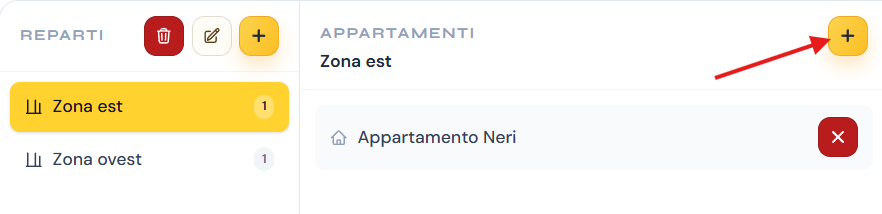
\includegraphics[width=0.8\textwidth]{./img/assegna_appart.png}
            \caption{Pulsante di aggiunta appartamento nella sezione del reparto}
        \end{figure}
    \item Selezionare l'appartamento da assegnare tra quelli disponibili;
        \begin{figure}[H]
            \centering
            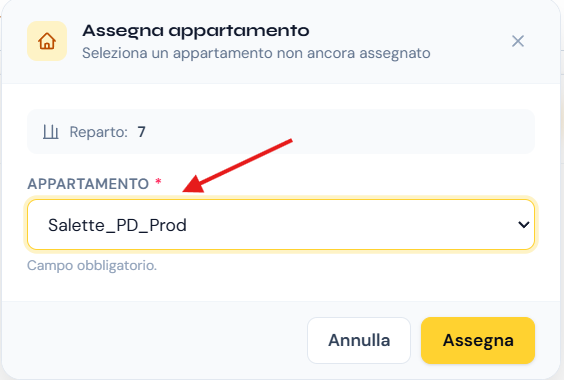
\includegraphics[width=0.5\textwidth]{./img/assegna_app_scegli.png}
            \caption{Selezione dell'appartamento da assegnare al reparto}
        \end{figure}
    \item Premere \textbf{Assegna}. Il Sistema registra l'assegnazione e 
          aggiorna l'elenco degli appartamenti del reparto.
        \begin{figure}[H]
            \centering
            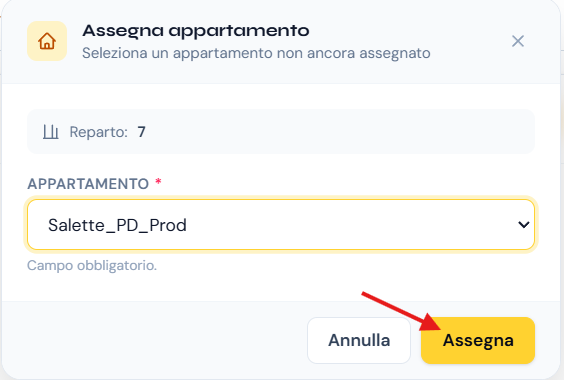
\includegraphics[width=0.5\textwidth]{./img/assegna_appartamento_rep.png}
            \caption{Conferma dell'assegnazione dell'appartamento al reparto}
        \end{figure}
\end{enumerate}

\subsubsection{Assegnare un Operatore Sanitario ad un reparto}
\begin{enumerate}
    \item Dalla sezione \textbf{Gestione Reparti}, selezionare il reparto desiderato;
    \item Selezionare la sezione \textbf{Operatori} e premere '+';
        \begin{figure}[H]
            \centering
            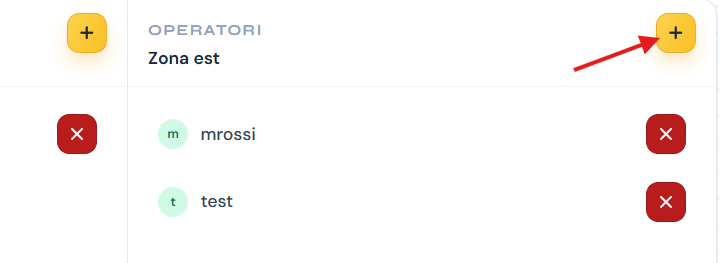
\includegraphics[width=0.5\textwidth]{./img/assegna_operatore.png}
            \caption{Pulsante di aggiunta operatore nella sezione del reparto}
        \end{figure}
    \item Selezionare l'Operatore Sanitario da assegnare tra quelli disponibili;
        \begin{figure}[H]
            \centering
            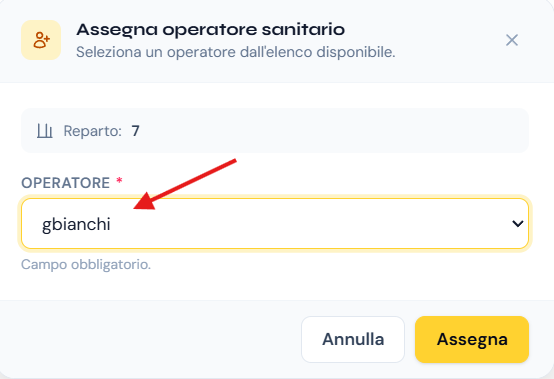
\includegraphics[width=0.5\textwidth]{./img/assegna_operatore_scegli.png}
            \caption{Selezione dell'Operatore Sanitario da assegnare al reparto}
        \end{figure}
    \item Premere \textbf{Assegna}. Il Sistema registra l'assegnazione.
        \begin{figure}[H]
            \centering
            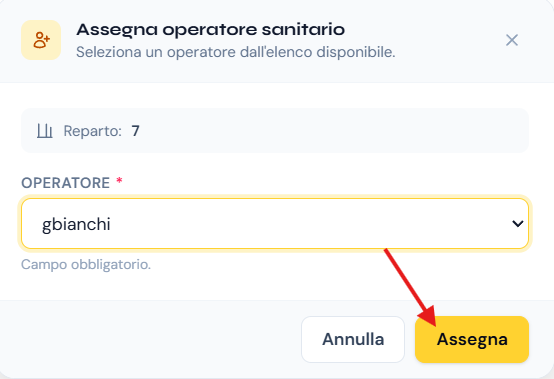
\includegraphics[width=0.5\textwidth]{./img/assegna_reparto.png}
            \caption{Conferma dell'assegnazione dell'Operatore Sanitario al reparto}
        \end{figure}
\end{enumerate}

\subsubsection{Rimuovere un appartamento da un reparto}
\begin{enumerate}
    \item Dalla sezione \textbf{Gestione Reparti}, selezionare il reparto desiderato;
    \item Nella sezione \textbf{Appartamenti}, premere il pulsante \textbf{X} 
    rosso accanto all'appartamento da rimuovere;

    \begin{figure}[H]
        \centering
        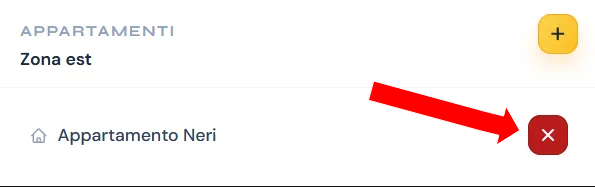
\includegraphics[width=0.6\textwidth]{img/rimozione_appartamento.png}
        \caption{Pulsante di rimozione appartamento dalla sezione del reparto}
    \end{figure}

    \item Confermare la rimozione premendo \textbf{Rimuovi} nel dialogo 
    di conferma;

    \begin{figure}[H]
        \centering
        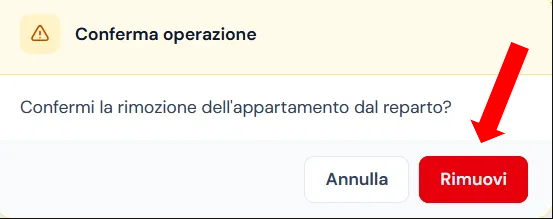
\includegraphics[width=0.6\textwidth]{img/conferma_rimozione_appartamento.png}
        \caption{Dialogo di conferma rimozione dell'appartamento dal reparto}
    \end{figure}

    \item Il Sistema rimuove l'appartamento dal reparto e aggiorna 
    l'elenco degli appartamenti associati.
\end{enumerate}

\subsubsection{Rimuovere un Operatore Sanitario da un reparto}
\begin{enumerate}
    \item Dalla sezione \textbf{Gestione Reparti}, selezionare il reparto desiderato;
    \item Nella sezione \textbf{Operatori}, premere il pulsante \textbf{X} 
    rosso accanto all'Operatore Sanitario da rimuovere;

    \begin{figure}[H]
        \centering
        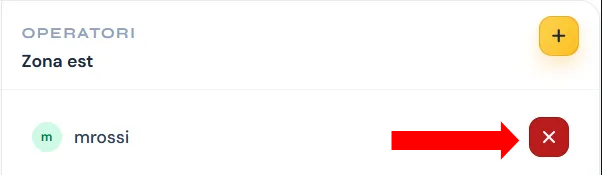
\includegraphics[width=0.6\textwidth]{img/eliminazione_os}
        \caption{Pulsante di rimozione Operatore Sanitario dalla sezione del reparto}
    \end{figure}

    \item Confermare la rimozione premendo \textbf{Rimuovi} nel dialogo 
    di conferma;

    \begin{figure}[H]
        \centering
        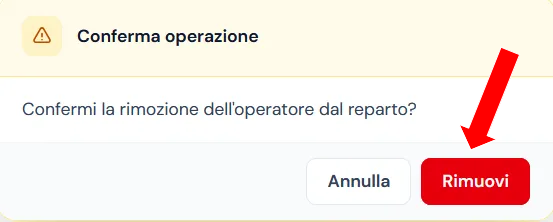
\includegraphics[width=0.6\textwidth]{img/conferma_rimozione_os.png}
        \caption{Dialogo di conferma rimozione dell'Operatore Sanitario dal reparto}
    \end{figure}

    \item Il Sistema rimuove l'Operatore Sanitario dall'appartamento e aggiorna 
    l'elenco degli operatori associati.
\end{enumerate}

\subsubsection{Eliminare un reparto}
\begin{enumerate}
    \item Dalla sezione \textbf{Gestione Reparti}, selezionare il reparto 
    da eliminare;
    \item Premere il pulsante \textbf{cestino} rosso nella sezione 
    \textbf{Reparti};

    \begin{figure}[H]
        \centering
        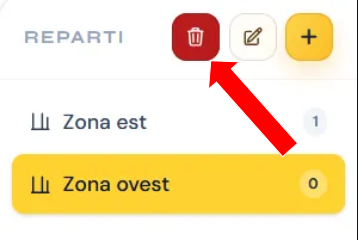
\includegraphics[width=0.4\textwidth]{img/eliminazione_reparto.png}
        \caption{Pulsante di eliminazione di un reparto}
    \end{figure}

    \item Confermare l'eliminazione premendo \textbf{Conferma} nel dialogo 
    di conferma;

    \begin{figure}[H]
        \centering
        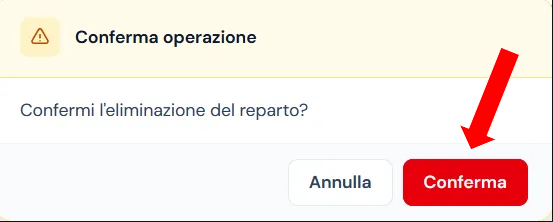
\includegraphics[width=0.6\textwidth]{img/conferma_rimozione_reparto.png}
        \caption{Dialogo di conferma eliminazione del reparto}
    \end{figure}

    \item Il Sistema elimina il reparto e lo rimuove dall'elenco 
    dei reparti configurati.
\end{enumerate}

\subsection{Gestire gli utenti}
\subsubsection{Visualizzare l'elenco degli Operatori Sanitari}
\begin{enumerate}
    \item Dal menu principale, selezionare la voce \textbf{Gestione Utenti};
        \begin{figure}[H]
            \centering
            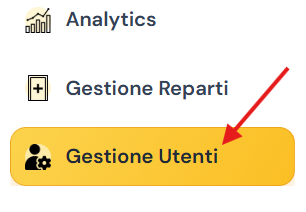
\includegraphics[width=0.3\textwidth]{./img/voce_gestione_utenti.png}
            \caption{Voce Gestione Utenti nel menu principale}
        \end{figure}
    \item Il Sistema mostra l'elenco degli Operatori Sanitari registrati. 
          Per ogni utente sono visibili:
          \begin{itemize}
              \item Il \textbf{nome};
              \item il \textbf{cognome};
              \item lo \textbf{username}.
          \end{itemize}
        \begin{figure}[H]
            \centering
            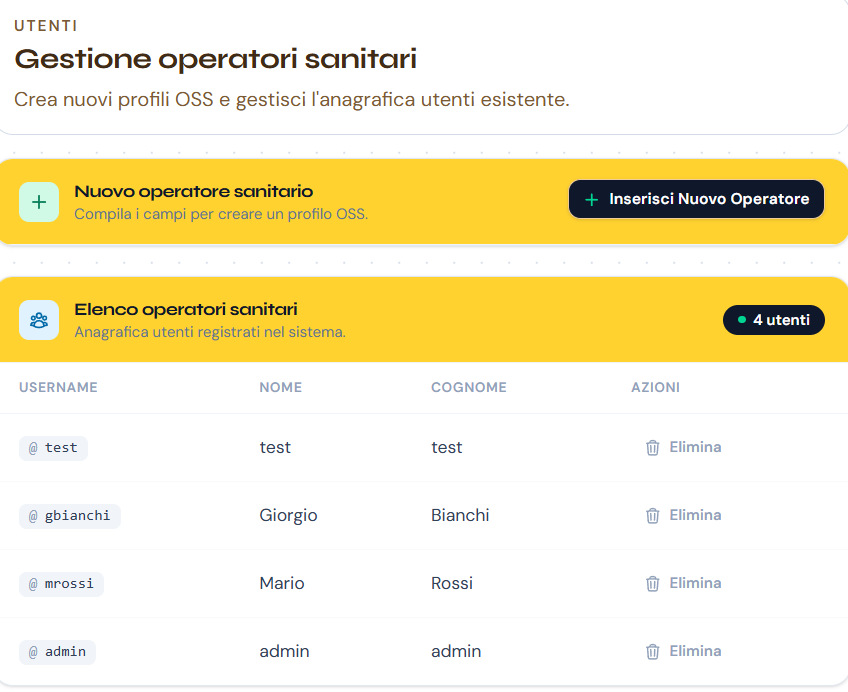
\includegraphics[width=0.6\textwidth]{./img/gestione_utenti_schermata.png}
            \caption{Schermata Gestione Utenti con l'elenco degli Operatori Sanitari}
        \end{figure}
\end{enumerate}

\subsubsection{Creare un nuovo Operatore Sanitario}
\begin{enumerate}
    \item Dalla sezione \textbf{Gestione Utenti}, premere il pulsante \textbf{Inserisci Nuovo Operatore};
        \begin{figure}[H]
            \centering
            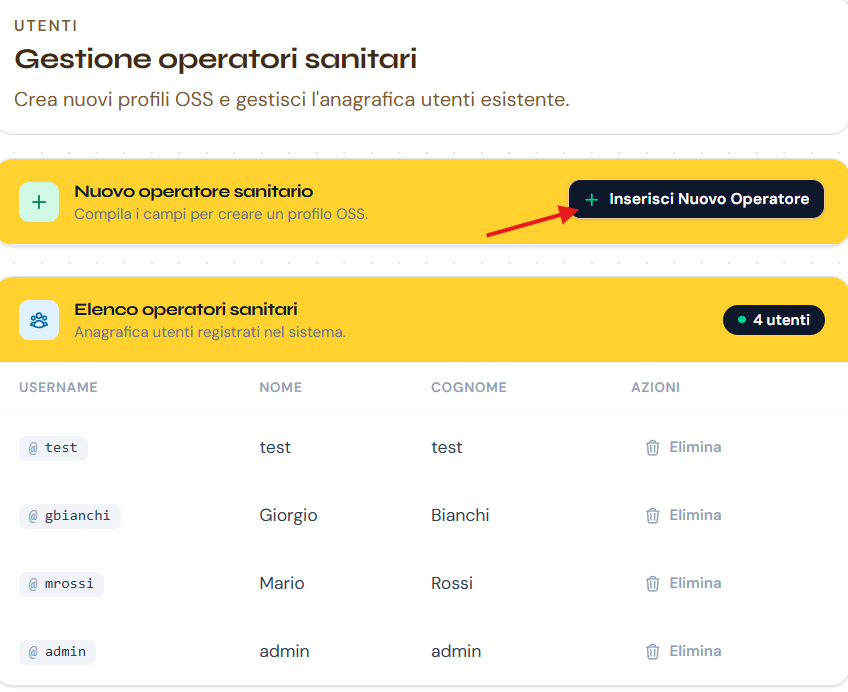
\includegraphics[width=0.6\textwidth]{./img/inserisci_nuovo_operatore.png}
            \caption{Pulsante Inserisci Nuovo Operatore nella sezione Gestione Utenti}
        \end{figure}
    \item Inserire il \textbf{nome}, il \textbf{cognome} e lo \textbf{username} 
          del nuovo Operatore Sanitario, quindi premere \textbf{Crea Utente}.
        \begin{figure}[H]
            \centering
            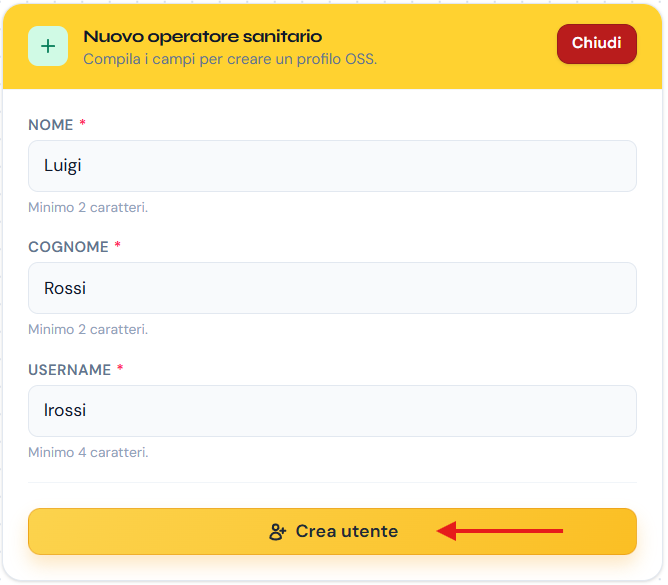
\includegraphics[width=0.6\textwidth]{./img/nuovo_oss.png}
            \caption{Form di creazione di un nuovo Operatore Sanitario}
        \end{figure}
    \item Il Sistema genera automaticamente una password provvisoria 
    da consegnare all'operatore;
        \begin{figure}[H]
            \centering
            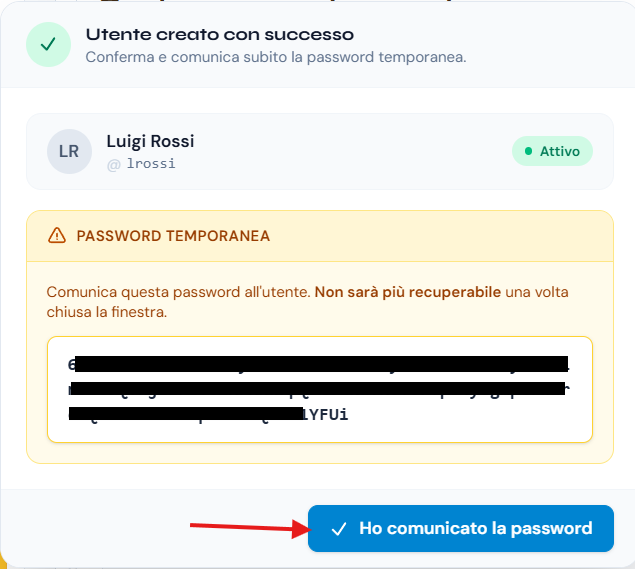
\includegraphics[width=0.6\textwidth]{./img/ho_comunicato_pass.png}
            \caption{Schermata con la password provvisoria generata per il nuovo Operatore Sanitario}
        \end{figure}
    \item Premere \textbf{Ho comunicato la password} per confermare. Il Sistema registra il 
          nuovo Operatore Sanitario e lo aggiunge all'elenco.
\end{enumerate}
Al primo accesso, l'Operatore Sanitario dovrà sostituire la password temporanea
con una personale, seguendo la procedura descritta nella Sezione \ref{sec:primo-accesso}.

\subsubsection{Eliminare un Operatore Sanitario}
\begin{enumerate}
    \item Dalla sezione \textbf{Gestione Utenti}, individuare l'Operatore Sanitario 
          da eliminare;
    \item Premere il pulsante \textbf{Elimina} accanto all'utente;
        \begin{figure}[H]
            \centering
            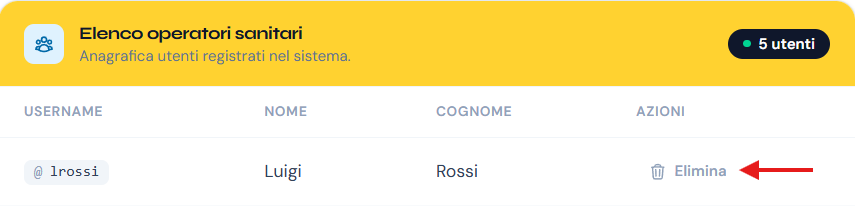
\includegraphics[width=0.6\textwidth]{./img/elimina_oss.png}
            \caption{Pulsante Elimina per un Operatore Sanitario}
        \end{figure}
    \item Confermare l'eliminazione premendo \textbf{Elimina} nel dialogo 
          di conferma.
        \begin{figure}[H]
            \centering
            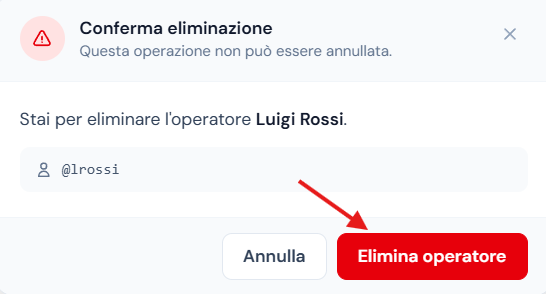
\includegraphics[width=0.5\textwidth]{./img/conferma_elimina_oss.png}
            \caption{Dialogo di conferma eliminazione dell'Operatore Sanitario}
        \end{figure}
    \item Il Sistema rimuove l'Operatore Sanitario dal Sistema.
\end{enumerate}

\section{Utente Operatore Sanitario: Guida all'utilizzo}
\subsection{Accesso}
\label{sec:accesso}
\begin{enumerate}
    \item Inserire le proprie credenziali nei campi \textbf{Username} e \textbf{Password};
    \item Premere \textbf{Accedi}. Il Sistema verifica le credenziali e reindirizza 
    alla \textit{Dashboard}.
        \begin{figure}[H]
            \centering
            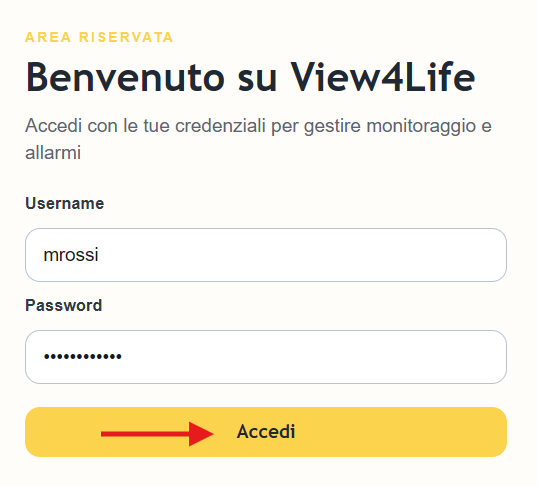
\includegraphics[width=0.5\textwidth]{./img/accesso.png}
            \caption{Schermata di accesso}
        \end{figure}
\end{enumerate}

\subsection{Primo accesso come Operatore Sanitario}
\label{sec:primo-accesso}
\begin{enumerate}
    \item Ottenere le credenziali provvisorie (username e password temporanea) 
          dall'\admin;
    \item Inserire le credenziali nella schermata di login e premere \textbf{Accedi};
        \begin{figure}[H]
            \centering
            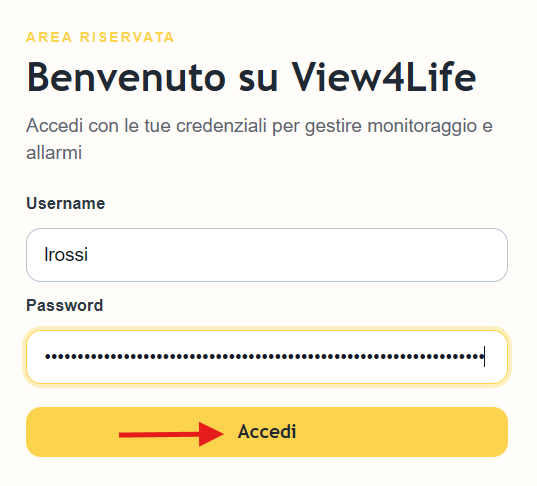
\includegraphics[width=0.5\textwidth]{./img/accedi_credenziali_temp.png}
            \caption{Accesso con credenziali temporanee}
        \end{figure}
    \item Il Sistema riconosce che si tratta del primo accesso e reindirizza 
          alla schermata di cambio password;
    \item Inserire la password temporanea nel campo \textbf{Password attuale};
    \item Inserire la nuova password nel campo \textbf{Nuova password};
    \item Premere \textbf{Conferma e continua}. Il Sistema aggiorna le credenziali e reindirizza 
    alla \textit{Dashboard}.
        \begin{figure}[H]
            \centering
            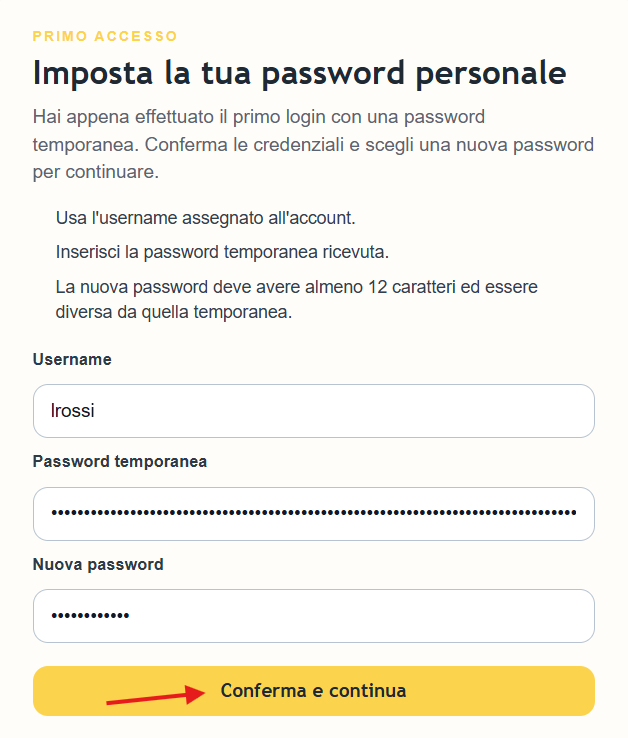
\includegraphics[width=0.5\textwidth]{./img/nuova_pass_oss.png}
            \caption{Schermata di cambio password al primo accesso}
        \end{figure}
\end{enumerate}

\subsection{Visualizzare la \textit{Dashboard}}
\begin{enumerate}
    \item Dal menu principale, selezionare la voce \textit{\textbf{Dashboard}};
        \begin{figure}[H]
            \centering
            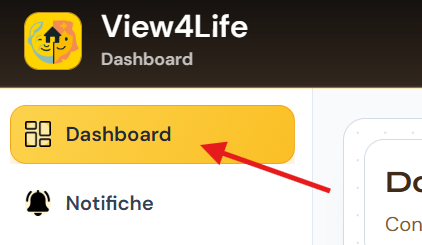
\includegraphics[width=0.4\textwidth]{./img/vai_dashboard.png}
            \caption{Voce Dashboard nel menu principale}
        \end{figure}
    \item Il Sistema mostra la \textit{Dashboard}, che include sempre il modulo
          \textbf{Gestione Allarmi} e i seguenti moduli:
          \begin{itemize}
              \item Statistiche Allarmi;
              \item Analisi Consumi;
              \item Struttura appartamento.
          \end{itemize}
        \begin{figure}[H]
            \centering
            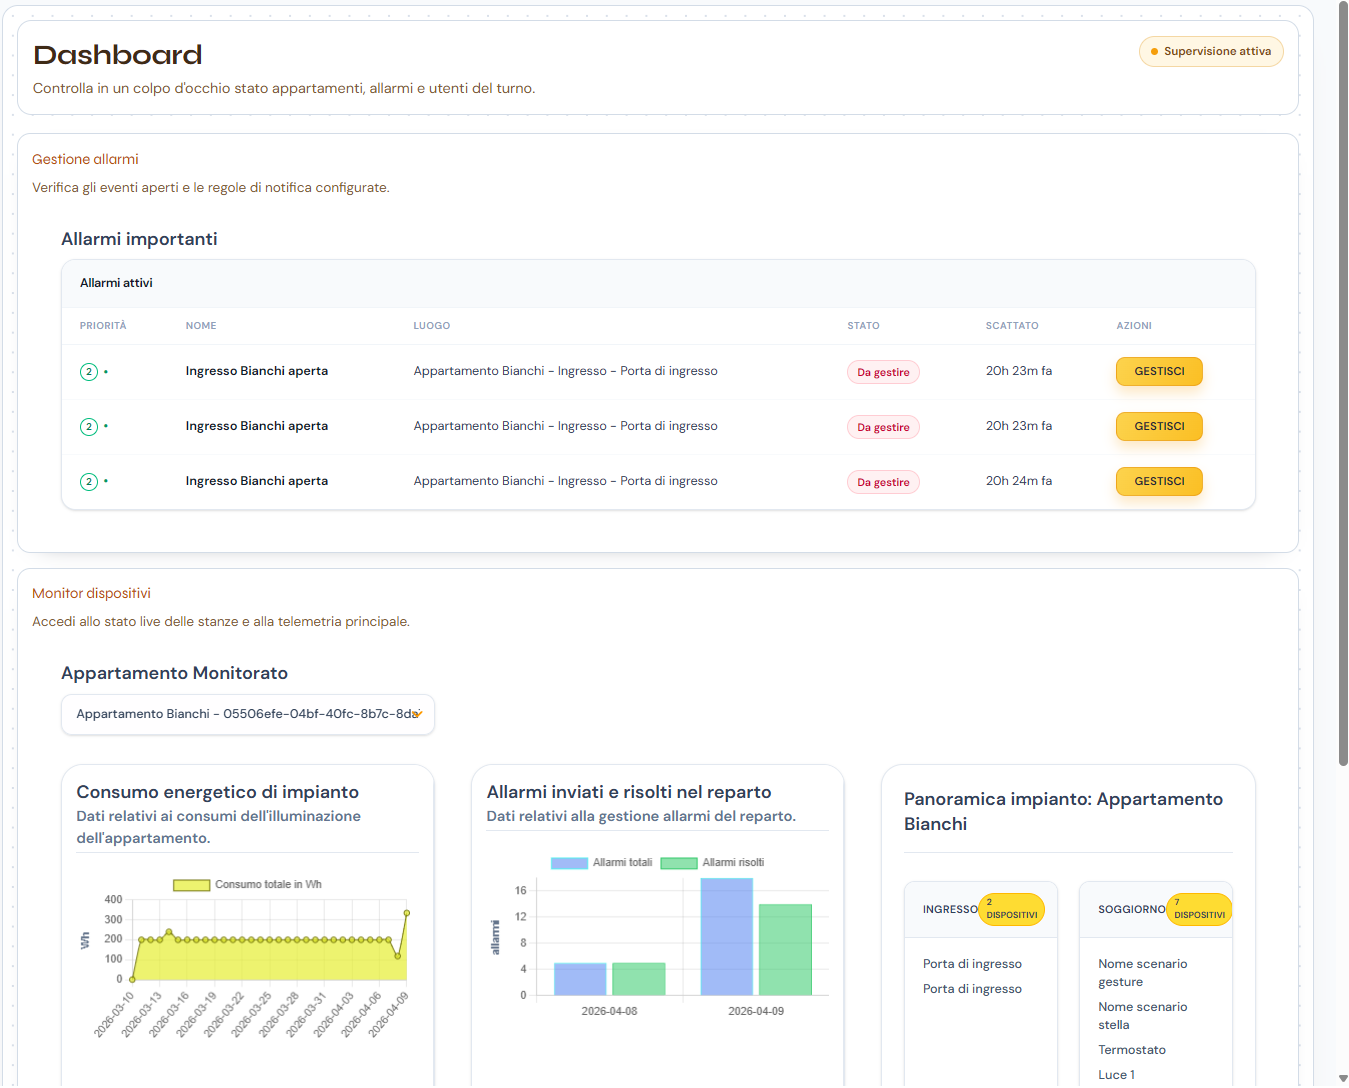
\includegraphics[width=\textwidth]{./img/dashboard.png}
            \caption{Schermata principale della Dashboard}
        \end{figure}
\end{enumerate}

\subsection{Gestire le notifiche}
\subsubsection{Visualizzare le notifiche}
\begin{enumerate}
    \item Dal menu principale, selezionare la voce \textbf{Notifiche}.
        \begin{figure}[H]
            \centering
            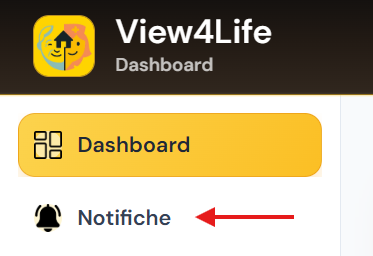
\includegraphics[width=0.4\textwidth]{./img/voce_notifiche.png}
            \caption{Voce Notifiche nel menu principale}
        \end{figure}
    \item Il Sistema mostra l'elenco delle notifiche. Per ogni notifica sono visibili:
          \begin{itemize}
              \item Il \textbf{titolo} della notifica;
              \item il \textbf{tempo trascorso} dall'invio.
          \end{itemize}
        \begin{figure}[H]
            \centering
            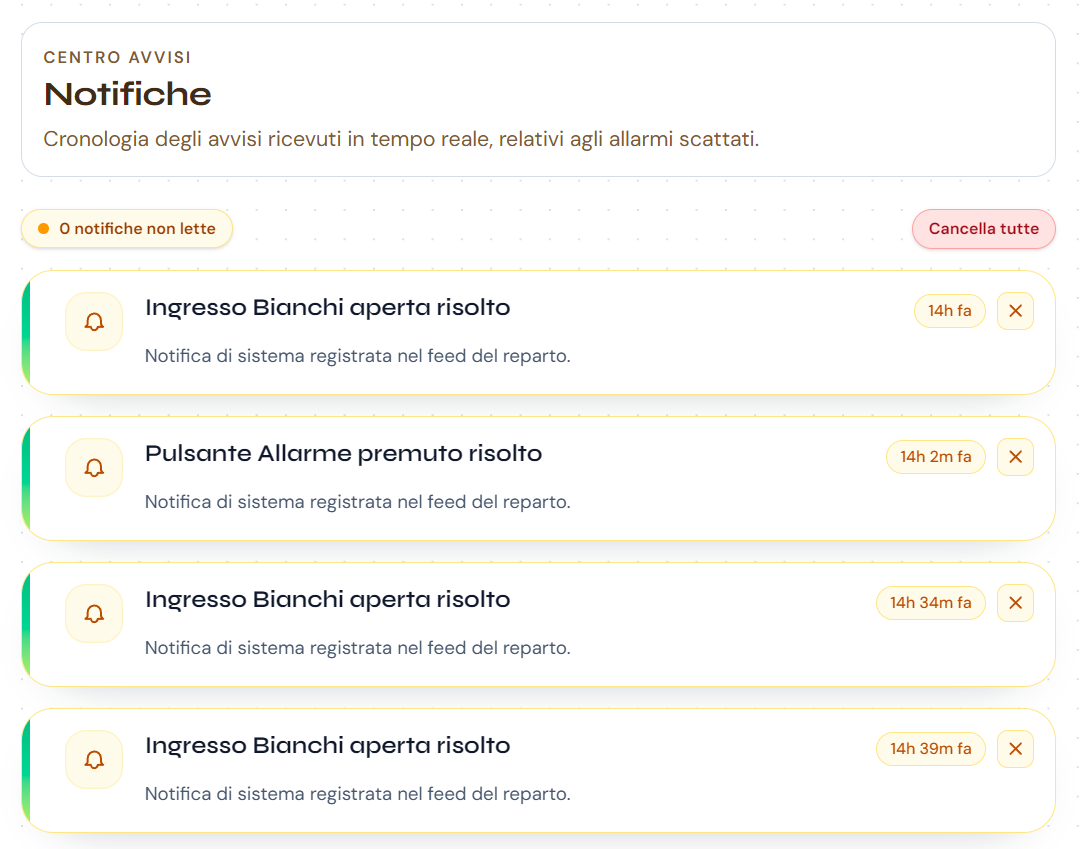
\includegraphics[width=0.8\textwidth]{./img/elenco_notifiche.png}
            \caption{Elenco delle notifiche}
        \end{figure}
\end{enumerate}

\subsubsection{Eliminare le notifiche}
\begin{enumerate}
    \item Dal menu principale, selezionare la voce \textbf{Notifiche};
    \item Individuare la notifica da eliminare nell'elenco;
    \item Premere il pulsante \textbf{Elimina} accanto alla notifica;
        \begin{figure}[H]
            \centering
            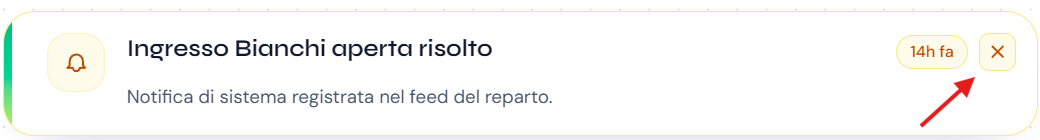
\includegraphics[width=0.7\textwidth]{./img/elimina_notifica.png}
            \caption{Pulsante Elimina per una singola notifica}
        \end{figure}
    \item Se si vogliono eliminare tutte le notifiche, premere il pulsante \textbf{Cancella tutte};
        \begin{figure}[H]
            \centering
            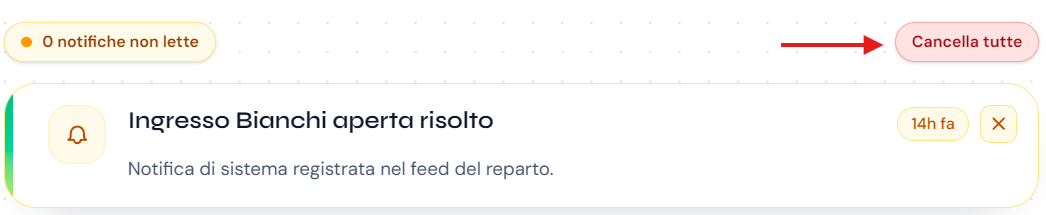
\includegraphics[width=0.7\textwidth]{./img/elimina_tutte_notifiche.png}
            \caption{Pulsante Cancella tutte le notifiche}
        \end{figure}
    \item Il Sistema rimuove la notifica dall'elenco.
\end{enumerate}

\subsection{Gestire i dispositivi di un appartamento}
\subsubsection{Visualizzare i dispositivi}
\begin{enumerate}
    \item Dal menu principale, selezionare la voce \textbf{Dispositivi};
        \begin{figure}[H]
            \centering
            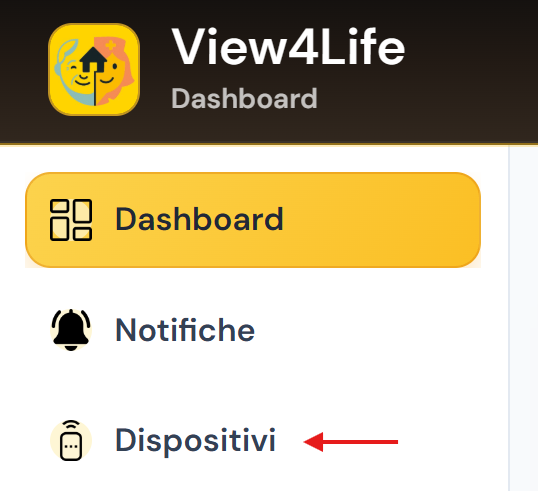
\includegraphics[width=0.4\textwidth]{./img/voce_dispositivi.png}
            \caption{Voce Dispositivi nel menu principale}
        \end{figure}
    \item Selezionare l'appartamento desiderato;
        \begin{figure}[H]
            \centering
            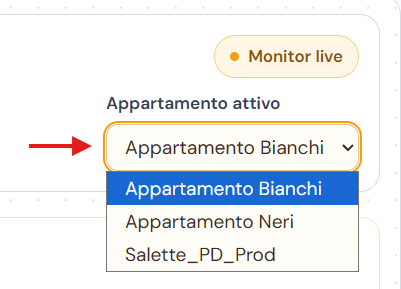
\includegraphics[width=0.4\textwidth]{./img/selettore_appartamento_dispositivi.png}
            \caption{Selettore appartamento nella sezione Dispositivi}
        \end{figure}
    \item Il Sistema mostra la vista dell'appartamento, con l'elenco delle stanze; 
    \item Il Sistema mostra l'elenco dei dispositivi suddivisi per stanza.\\
          Per ogni dispositivo sono visibili:
          \begin{itemize}
              \item Il \textbf{nome} del dispositivo;
              \item Il \textbf{tipo};
              \item L'\textbf{endpoint} associato;
              \item lo \textbf{stato} attuale;
              \item un selettore di \textbf{valore};
              \item l' \textbf{azione} di scrittura.
          \end{itemize}
        \begin{figure}[H]
            \centering
            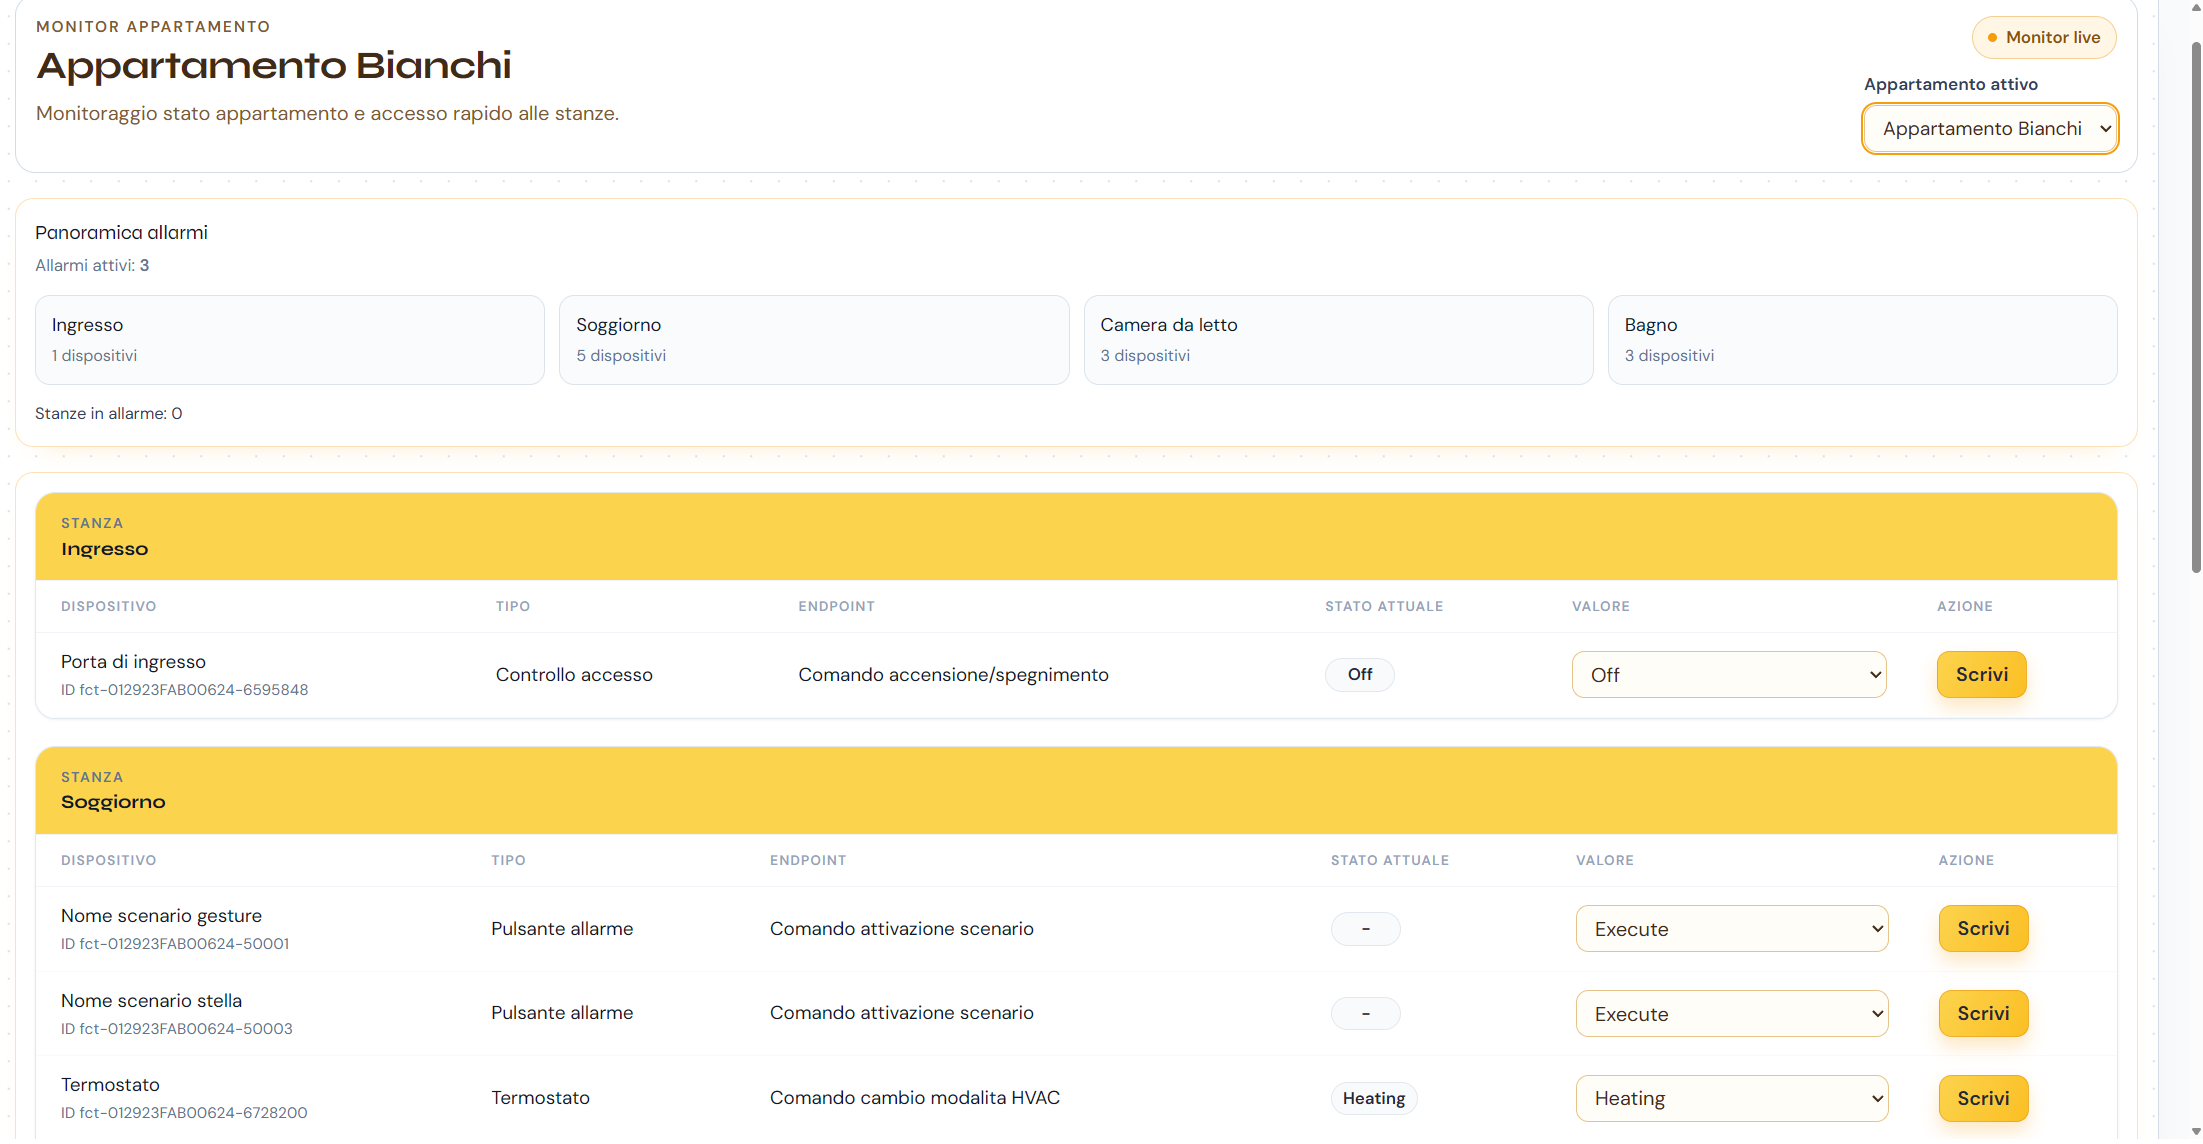
\includegraphics[width=\textwidth]{./img/elenco_dispositivi.png}
            \caption{Elenco dei dispositivi suddivisi per stanza}
        \end{figure}
\end{enumerate}

\subsubsection{Modificare lo stato dei dispositivi}
\begin{enumerate}
    \item Visualizzare i dispositivi della stanza seguendo i passi descritti 
          nella sezione precedente;
    \item Individuare il dispositivo da modificare;
    \item Selezionare l'azione desiderata tra quelle disponibili per il dispositivo;
        \begin{figure}[H]
            \centering
            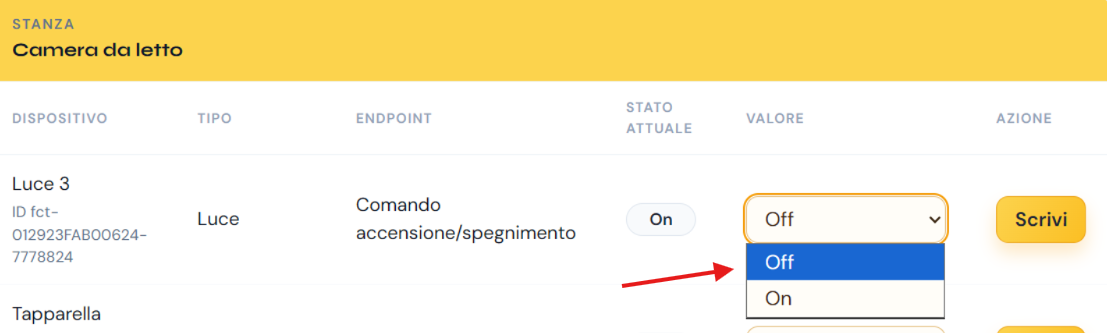
\includegraphics[width=\textwidth]{./img/opzioni_disp.png}
            \caption{Opzioni disponibili per la modifica di un dispositivo}
        \end{figure}
    \item Dopo aver selezionato il nuovo stato, premere \textbf{Scrivi};
        \begin{figure}[H]
            \centering
            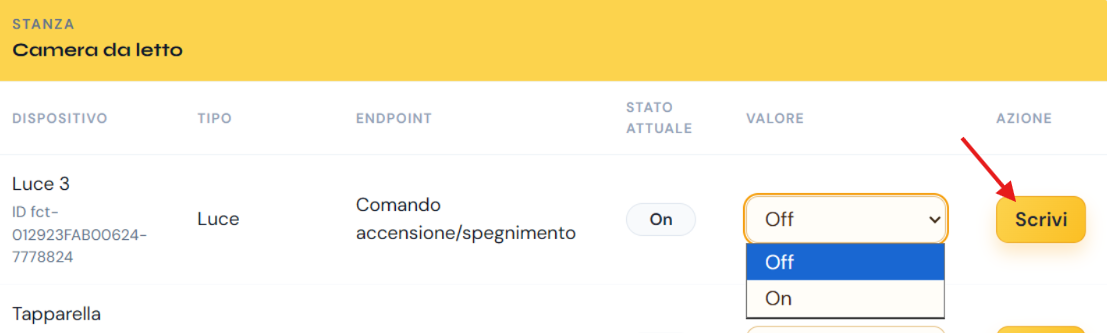
\includegraphics[width=\textwidth]{./img/scrivi.png}
            \caption{Pulsante Scrivi per confermare la modifica del dispositivo}
        \end{figure}
    \item Il Sistema invia il comando al dispositivo e comunica all'utente il cambio di stato;
        \begin{figure}[H]
            \centering
            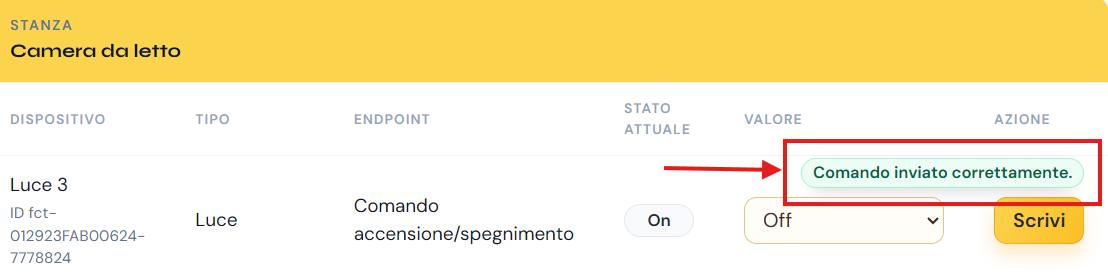
\includegraphics[width=\textwidth]{./img/comando_corr.png}
            \caption{Conferma dell'avvenuto cambio di stato del dispositivo}
        \end{figure}
    \item Per poter visualizzare il nuovo stato del dispositivo è necessario ricaricare la pagina.
\end{enumerate}

\subsection{Gestire gli allarmi attivi}
\subsubsection{Visualizzare gli allarmi attivi}
Il modulo \textbf{Gestione Allarmi} è sempre visibile nella Dashboard e dalla voce del menu principale \textbf{Gestione Allarmi} e presenta
l'elenco degli allarmi correntemente attivi. Per ogni allarme sono mostrati:
\begin{itemize}
    \item Il \textbf{segnale di pericolo} (indicatore visivo del livello di priorità);
    \item il \textbf{nome} dell'allarme;
    \item il \textbf{luogo} in cui è scattato l'allarme;
    \item il \textbf{tempo trascorso} dallo scatto dell'allarme.
\end{itemize}
\begin{figure}[H]
    \centering
    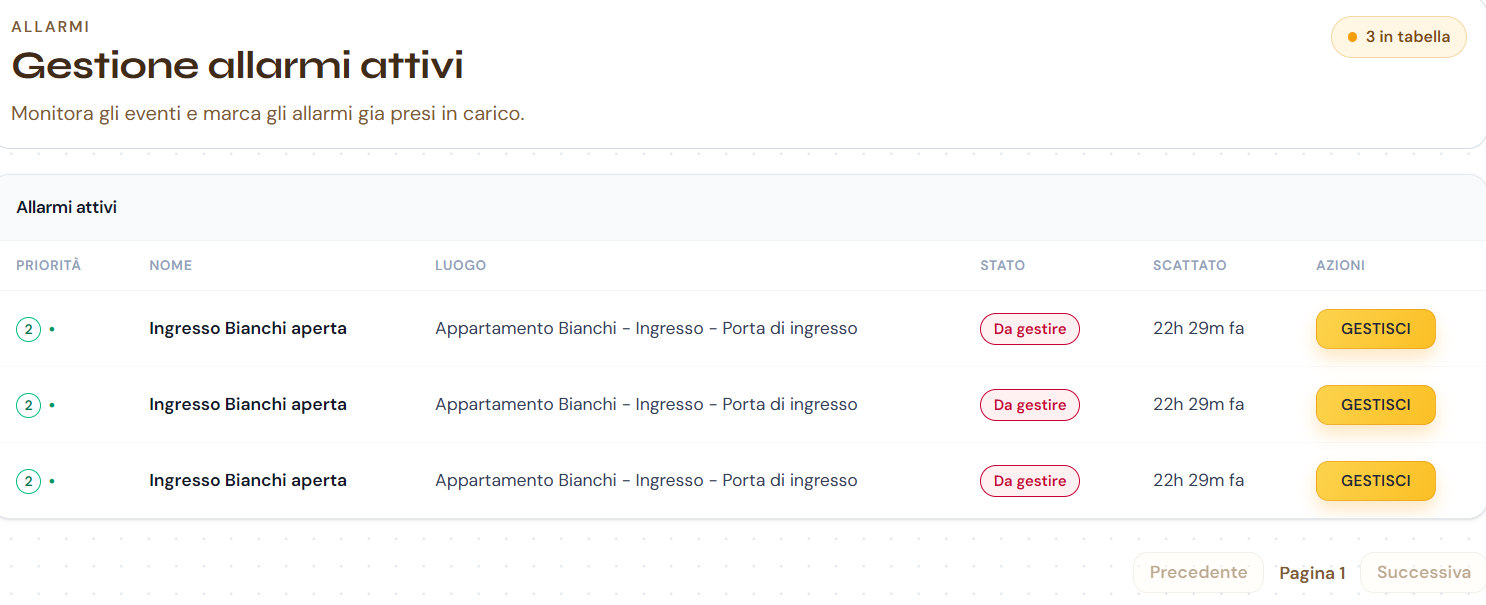
\includegraphics[width=\textwidth]{./img/gestione-allarmi.png}
    \caption{Modulo Gestione Allarmi con elenco degli allarmi attivi}
\end{figure}

\subsubsection{Risolvere un allarme attivo}
\begin{enumerate}
    \item Dal menu principale, selezionare la voce \textbf{Gestione Allarmi};
    \item Individuare l'allarme da risolvere;
    \item Premere il pulsante \textbf{Gestisci} accanto all'allarme;
        \begin{figure}[H]
            \centering
            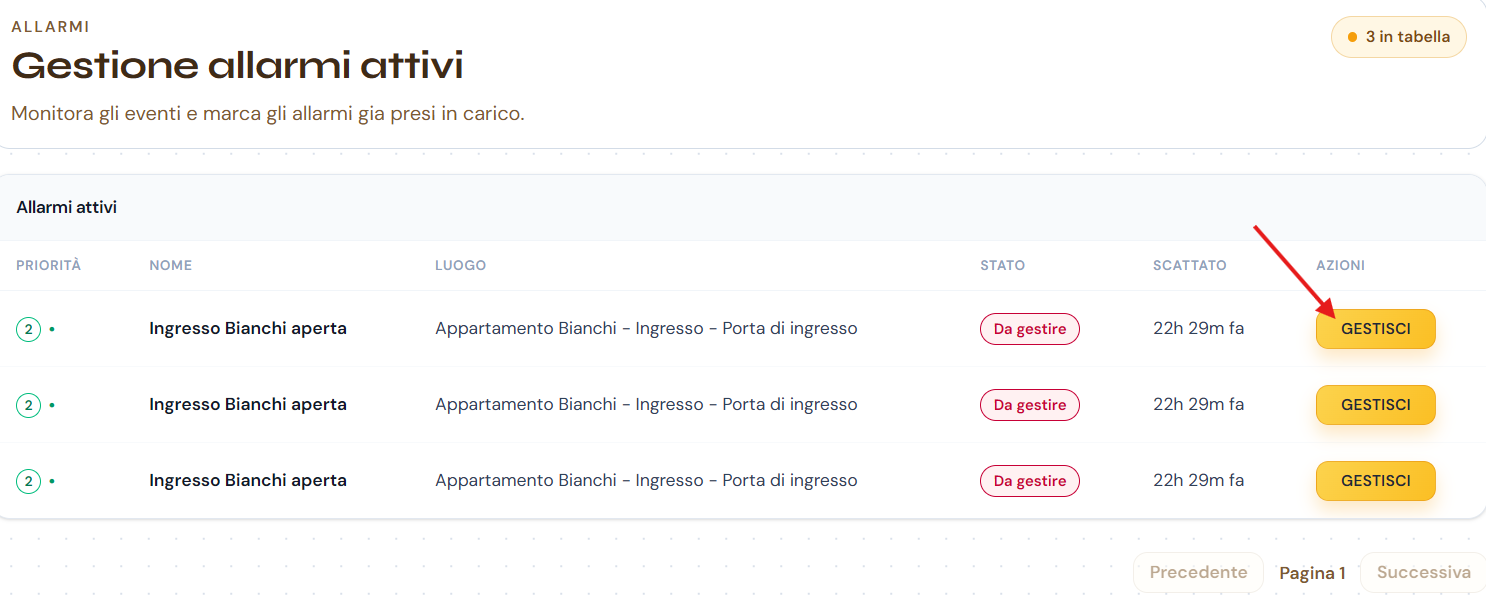
\includegraphics[width=\textwidth]{./img/gestisci.png}
            \caption{Pulsante Gestisci per la risoluzione di un allarme}
        \end{figure}
    \item Il Sistema contrassegna l'allarme come risolto e lo rimuove dall'elenco degli allarmi attivi.
\end{enumerate}

\subsubsection{Visualizzare lo storico degli allarmi risolti}
\begin{enumerate}
    \item Dal menu principale, selezionare la voce \textbf{Storico Allarmi};
        \begin{figure}[H]
            \centering
            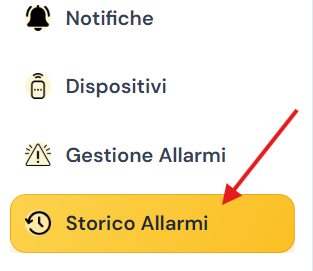
\includegraphics[width=0.4\textwidth]{./img/voce_storico_allarmi.png}
            \caption{Voce Storico Allarmi nel menu principale}
        \end{figure}
    \item Il Sistema mostra l'elenco degli allarmi contrassegnati come risolti. 
          Per ogni allarme sono visibili:
          \begin{itemize}
              \item Il \textbf{nome} dell'allarme;
              \item il \textbf{luogo} in cui è scattato;
              \item l' \textbf{orario di scatto};
              \item l' \textbf{orario di risoluzione};
              \item il \textbf{gestore} dell'allarme.
          \end{itemize}
        \begin{figure}[H]
            \centering
            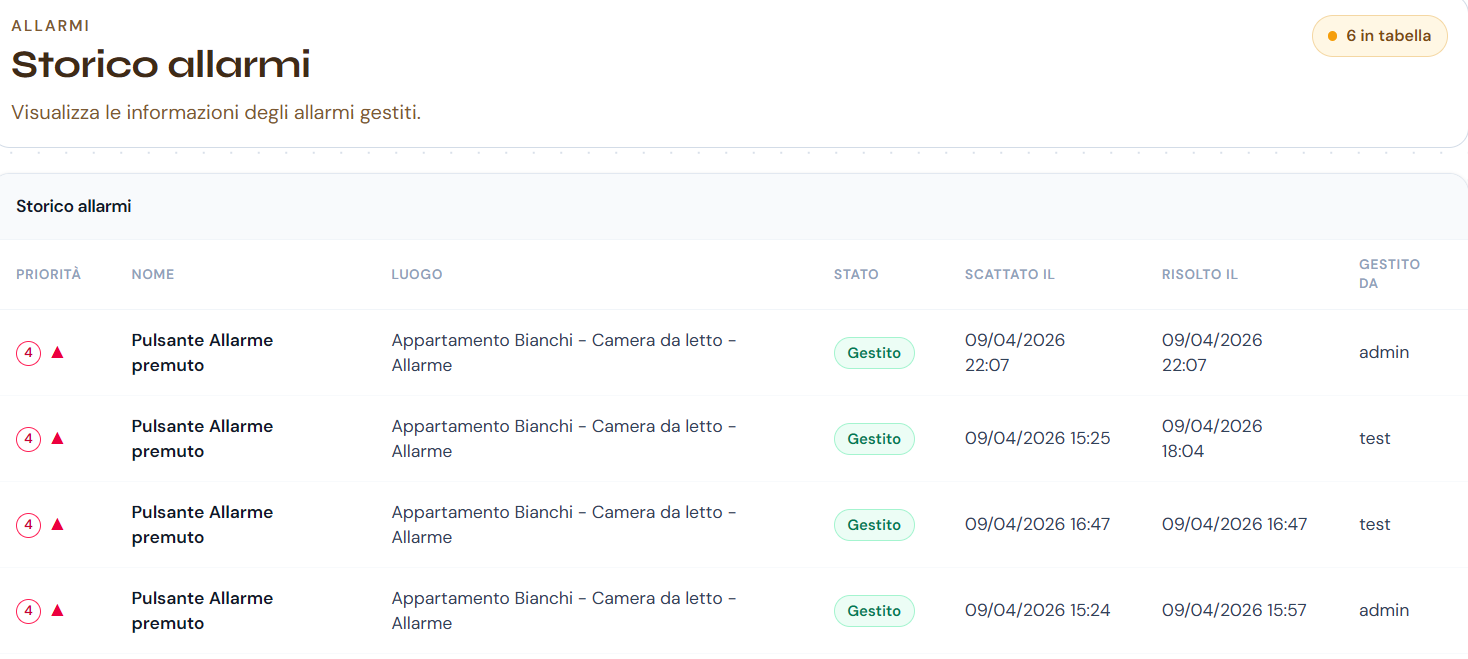
\includegraphics[width=\textwidth]{./img/storico_allarmi.png}
            \caption{Schermata Storico degli allarmi risolti}
        \end{figure}
\end{enumerate}

\subsection{Visualizzare le \textit{Analytics} di un appartamento}
\begin{enumerate}
    \item Dal menu principale, selezionare la voce \textbf{Analytics};
        \begin{figure}[H]
            \centering
            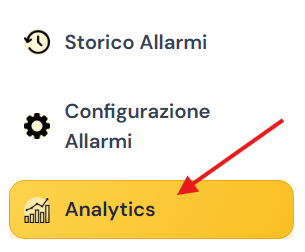
\includegraphics[width=0.4\textwidth]{./img/voce_analytics.png}
            \caption{Voce Analytics nel menu principale}
        \end{figure}
    \item Selezionare l'appartamento di cui si vogliono visualizzare le analytics;
        \begin{figure}[H]
            \centering
            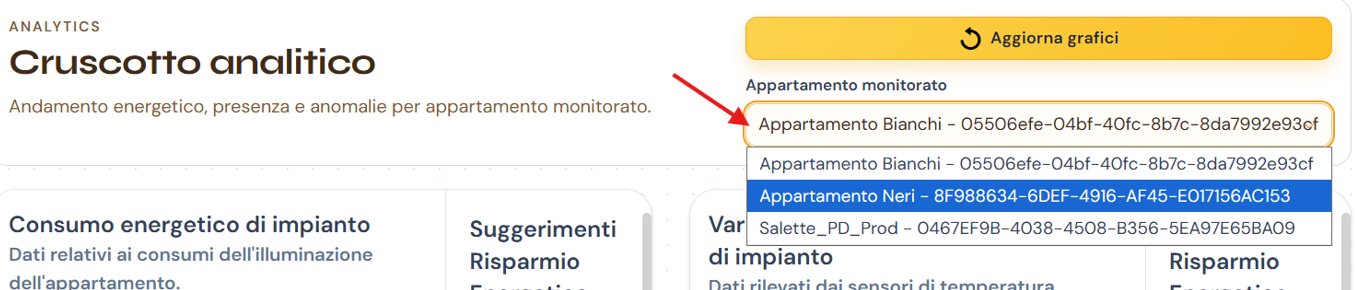
\includegraphics[width=\textwidth]{./img/analytics_sel_app.png}
            \caption{Selettore appartamento nella sezione Analytics}
        \end{figure}
    \item Il Sistema mostra i grafici relativi all'appartamento selezionato, tra cui:
          \begin{itemize}
              \item \textbf{Consumo energetico};
              \item \textbf{Anomalie dell'impianto};
              \item \textbf{Rilevamento di presenza};
              \item \textbf{Presenza prolungata};
              \item \textbf{Variazioni di temperatura};
              \item \textbf{Allarmi inviati e risolti};
              \item \textbf{Frequenza degli allarmi};
              \item \textbf{Frequenza delle cadute}.
          \end{itemize}
        \begin{figure}[H]
            \centering
            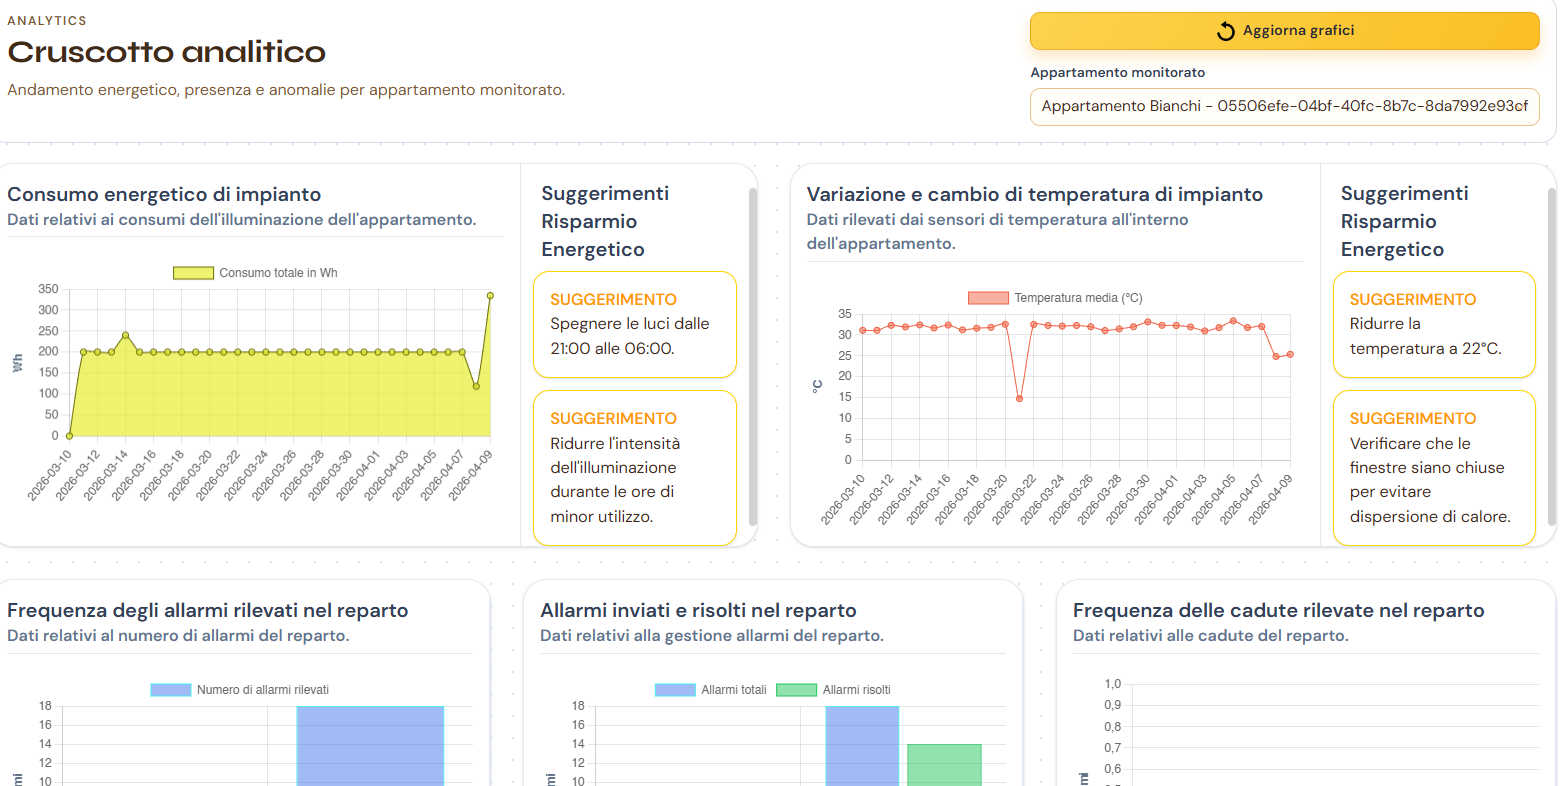
\includegraphics[width=\textwidth]{./img/analytics.png}
            \caption{Schermata Analytics con i grafici dell'appartamento selezionato}
        \end{figure}
\end{enumerate}

\section{Riferimento API}
La specifica OpenAPI del Sistema è disponibile alla seguente pagina: \url{https://view4life.me/api/docs}.

\section{Supporto Tecnico}
Il nostro team è disponibile per offrire supporto in caso di domande o problematiche legate al progetto. 
In presenza di difficoltà tecniche, dubbi sull'utilizzo delle funzionalità o problemi durante l'installazione, 
è possibile contattarci all'indirizzo snakebyteteam@gmail.com, descrivendo nella maniera più dettagliata possibile il problema.

\end{document}